\RequirePackage{plautopatch}
\RequirePackage[l2tabu, orthodox]{nag}

\documentclass[platex,dvipdfmx]{jlreq}			% for platex
% \documentclass[uplatex,dvipdfmx]{jlreq}		% for uplatex
\usepackage{graphicx}
\usepackage{bxtexlogo}
\usepackage{udline}
\usepackage{caption} 

\renewcommand{\baselinestretch}{1.2}

% Customize the caption font
\captionsetup{
    font={normalsize},  % Set the font size to normal
    labelfont={normalsize},    % Set the label font size to normal
    textfont={normalsize},     % Set the text font size to normal
    justification=centering, % Center the caption
}

\usepackage[backend=biber,style=chem-acs]{biblatex} % Load the biblatex package
\addbibresource{reference.bib} % Add the .bib file

\usepackage{titling} % Load the titling package
% Adjust the title position
\setlength{\droptitle}{-2.5cm} % Adjust this value as needed

\renewcommand{\figurename}{Fig.}
\renewcommand{\tablename}{Table}

\usepackage{float}

\title{酸化グラフェンアシストシリコン気相エッチングにおけるシート面内構造依存性の評価}

\author{機能構築学研究室 修士2回 後藤雄太}
\date{2024年06月28日}
\begin{document}
\maketitle

\section*{\ul{Introduction}}
グラファイトからグラフェンの分離が2004年に実証されて以来\supercite{novoselov_electric_2004},グラフェンはその優れた材料特性からトランジスタやガスセンサー,潤滑剤などへの応用が期待されている\supercite{schwierz_graphene_2010, lu_toward_2011, chen_hgii_2012, jin_lubrication_2023}.
しかし,単層かつ高品位なグラフェンを大量生産することは技術的に難しく,実用化に向けた低コスト・高効率なグラフェン作製プロセスの開発が求められている.
このグラフェンの生産方法として,グラファイトを酸化および,剥離して得られる酸化グラフェン(Graphene Oxide: GO)(Fig.\ref{fig:schematic_model}(a))を還元する手法が注目されてきた.
GOを還元する手法としては,熱還元\supercite{song_effect_2013}や化学還元\supercite{de_silva_highquality_2022},電気化学還元\supercite{shao_facile_2010}などがあるが,低消費エネルギーかつ,毒性の高い薬品(e.g. ヒドラジン)を用いない還元方法として光還元\supercite{matsumoto_photoreduction_2010}が挙げられる.
Tuらは波長 172 nmを有する真空紫外(Vacuum Ultra-Violet: VUV)光を高真空環境下でGOに照射することで,GOから酸素含有官能基(Oxygen-containing Functional Groups: OFGs)を除去することを可能とした\supercite{tu_reductive_2014}.
また,廣富らはGOを140 ${}^\circ$Cで加熱しながらVUV光照射によって還元することで,より欠陥の少ない酸化グラフェン還元体(reduced Graphene Oxide: rGO)を作製することに成功している\supercite{hirotomi_fabrication_2022}.\\
\indent
近年では,GOはグラフェン作製のための前駆体であるだけでなく,機能性材料として応用が進められている.
窪田らはGOをシリコン基板上に担持し,エッチャントに浸漬させるとGOで覆われたシリコンが優先的に溶解する触媒エッチングを提案した\supercite{kubota_chemical_2019}.
これはGOが触媒として過酸化水素や溶存酸素といった酸化剤の還元を促進することに起因している.
GOのエッジや粒界,空孔といった欠陥が酸化剤を吸着する\supercite{kamiya_graphene_2014}ため,酸化剤還元が促進されると窪田らは考察しており,また,液相の場合は酸化剤の還元反応が律速過程であることが明らかとなっている\supercite{kubota_chemical_2021}.
一方,これまでにも,GOだけでなくさまざまな触媒を用いた半導体ウェットエッチングが報告されてきた\supercite{wilhelm_ordered_2019, jeong_titanium_nitride_2019, gayrard_replacing_2021, yamamoto_mos_2024}.
特に,貴金属を用いたエッチング(Metal-assisted chemical etching: Macetch)はウェットエッチングにも拘らず,高い異方性を有する半導体微細構造を作製することが可能であるため,ドライエッチングに代わる半導体微細加工技術として注目を集めてきた(Fig.\ref{fig:schematic_model}(b))\supercite{huang_metal-assisted_2010, lianto_vertical_2012, li_deep_2014}.
しかし, Macetchの欠点として,貴金属が高価であること,そして残留金属が半導体に深い準位を形成し\supercite{tavendale_deep_1983},デバイス性能に悪影響を与える可能性があることが挙げられる.
それに対して,GOは簡易なプロセスで作製可能であり,また,VUV光での除去が容易である.
従来のGOを用いたエッチングでは,これまでに酸化剤に硝酸を使用することでエッチングの高速化や,エッチングメカニズムの解明が行われてきた\supercite{kubota_chemical_2021}.
それにもかかわらず,発生するガスによってGOが半導体基板からエッチャント中に剥離してしまうため,本手法では大面積を均一に加工することが困難とされてきた.
また,GO非被覆部のシリコンにナノ・メソスケールのポーラス構造が形成されることによる選択性の低下もシリコンナノワイヤやMEMSなどの単結晶シリコンが必要な応用には望ましくない.
窪田らはエッチャントを加熱することで蒸気にし,それをGO担持シリコン基板に暴露することで,GOの剥離を抑制することに成功した\supercite{kubota_vapor-phase_2022}(Fig.\ref{fig:schematic_model}(c)).\\
\indent
本研究では,この気相エッチングのメカニズムおよび律速過程を解明することを試みる.
GOおよびVUV光還元から得られたrGOが異なるシート面内構造を有することを利用して,構造欠陥がエッチング反応に与える影響を明らかにする.

\begin{figure}
    \centering
    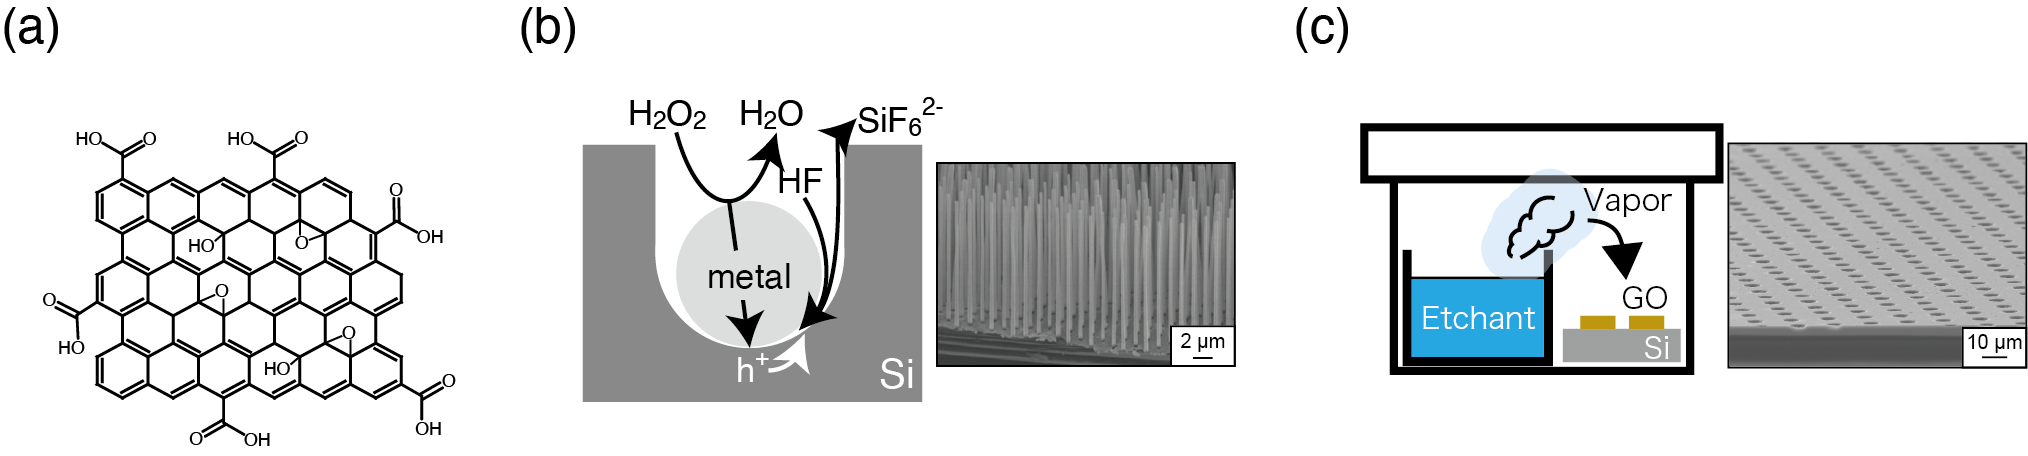
\includegraphics[width=155mm]{figures/figure1.png}
    \caption{A schematic image of (a) Graphene Oxide, (b) the mechanism of Macetch (left), and (c) the vapor etching process (left). SEM images of silicon processed by Macetch or GO-assisted etching are shown in (b) and (c) (both right), respectively.}
    \label{fig:schematic_model}
\end{figure}

\newpage
\section*{\ul{Experiment 1. Characterization of GO and rGO}}

\subsection*{\ul{Purpose of this experiment}}
酸化度およびシート面内構造の異なるGOをエッチング挙動の比較のために複数作製する.
GOならびに室温でのVUV光照射還元によって得られるrGO,そして140 ${}^\circ$Cで加熱しながらVUV光照射照射還元を行うことで得られるrGO\_140の評価をすることで,GO還元体の作製に成功したか確認する.

\subsection*{\ul{Experimental procedure}}
\begin{enumerate}
    \item 1 $\times$ 1 cm$^2$ Si (boron-doped p-type (100), 1 - 30 $\Omega\cdot$cm) substrates or Si substrate covered with a thermal oxide layer (boron-doped p-type (100), 90 nm SiO$_2$, 0.1 $\Omega\cdot$cm) were ultrasonically cleaned by acetone, ethanol, and Ultra Pure Water (UPW) for 30 min respectively and then cleaned by VUV (Xe) light irradiation for 20 min.
    \item GO (fabricated by chemically exfoliation method, a.k.a Hummers' method ) dispersion was spread onto the substrates by spin-coating (500 rpm for 15 s and then 2000 rpm for 150 s).
    \item The height of the GO sheets was observed by AFM (Atomic Force Microscope) and GO sheets were characterized by XPS (X-ray Photoelectron Spectroscopy) and Raman spectroscopy.
    \item The substrate with GO sheets was reduced by irradiation of VUV (Xe) light in a high vacuum ($<$ 10$^{-3}$ Pa) at room temperature or 140 ${}^\circ$C for 64 min.
    \item The height of the rGO or rGO\_140 sheets was observed by AFM and they were characterized by XPS and Raman spectroscopy as well.
\end{enumerate}

\subsection*{\ul{Results and discussion}}

\subsubsection*{\ul{AFM}}
Fig.\ref{fig:AFM}はそれぞれ酸化膜付きシリコン基板に担持した(a) GO, (b) rGO, (c) rGO\_140のAFM像である.
GOの厚さは約1.2 nmほどであり\supercite{tu_vacuum-ultraviolet_2015},VUV光照射によって得られたrGO,rGO\_140の厚さはその半分の0.6 nmほどと減少していた.
これはVUV光照射によってGOシート上に存在するOFGが除去されたためと推測できる.
140 ${}^\circ$Cでの加熱を併用したrGO\_140ではOFGだけでなく,吸着水の除去も進行すると考えられるが,rGOと比較して,さらにその厚さが減少するということは観察されなかった.
Pristineなグラフェンの厚さが0.34 nm程度であることから,VUV光照射では全てのOFGや吸着水を除去することはできなかったことが本結果から示唆された.

\begin{figure}
    \centering
    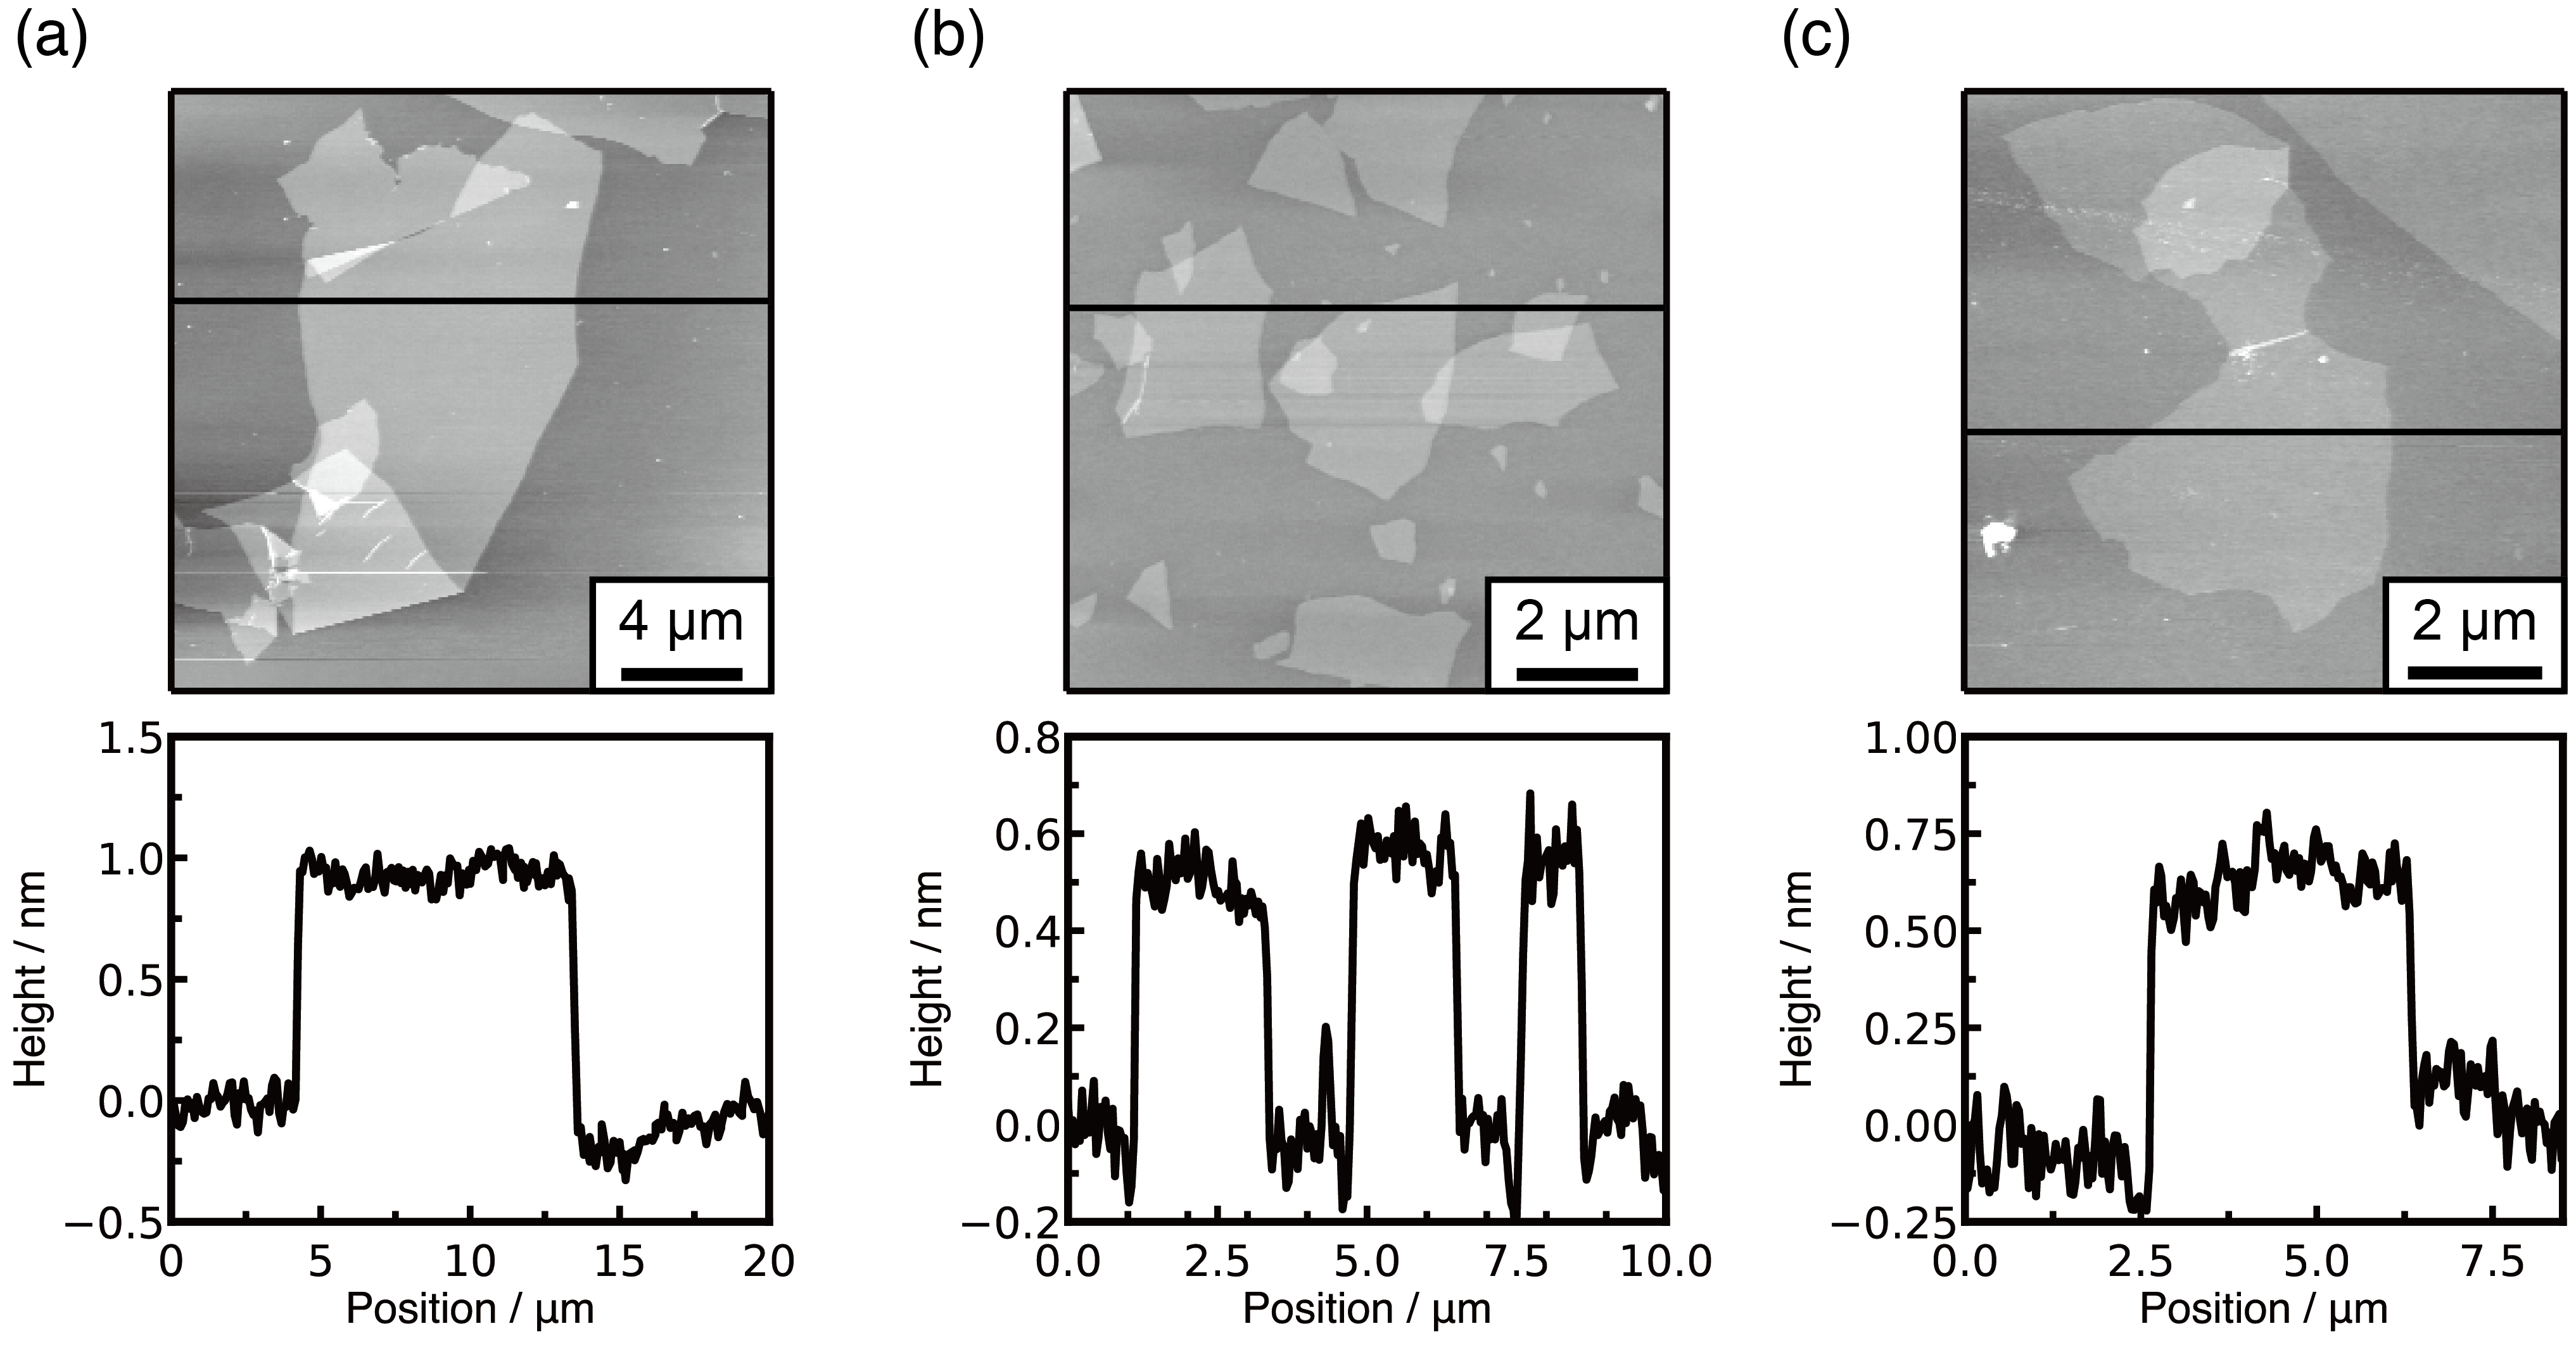
\includegraphics[width=150mm]{figures/figure2.png}
    \caption{AFM topographic images and cross-sectional profiles along the lines of (a) GO, (b) rGO, and (c) rGO\_140 on SiO$_2$ substrates.}
    \label{fig:AFM}
\end{figure}

\subsubsection*{\ul{XPS}}
Fig.\ref{fig:XPS}は各GOのC 1sスペクトルを示す ((a) GO, (b) rGO, (c) rGO\_140).
VUV光照射前後でのOFGの種類とその割合の変化を調べるため,C 1sスペクトルのピークを6つの成分で分離した\supercite{tu_vacuum-ultraviolet_2015}.
6つのピークはそれぞれ,C=C (284.4 eV, Full Width Half Maximum (FWHM) = 1.50 eV),C-C (285.0 eV, FWHM = 1.36 eV),C-OH (286.2 eV, FWHM = 1.46 eV), C-O-C (286.9 eV, FWHM = 1.24 eV), C=O (287.9 eV, FWHM = 1.57 eV), COOH (289.1 eV), FWHM = 1.41 eVとした.
Table1にそれぞれ分離したピークの面積比を示す.

\begin{table}[H]
    \centering
    \caption{$R_{\mathrm{O/C}}$ (unit: \%) of GO, rGO, and rGO\_140.}
    \label{tab:xps}
    \begin{tabular}{|c|c|c|c|c|c|c|c|}
        \hline
        ~        & $P_{\mathrm{C=C}}$ & $P_{\mathrm{C-C}}$ & $P_{\mathrm{C-OH}}$ & $P_{\mathrm{C-O-C}}$ & $P_{\mathrm{C=O}}$ & $P_{\mathrm{COOH}}$ & $R_{\mathrm{O/C}}$ \\ \hline
        GO       & 15.54              & 38.26              & 9.92                & 19.24                & 13.74              & 3.30                & 39.9 \\ \hline
        rGO      & 20.27              & 45.58              & 20.81               & 2.10                 & 6.73               & 4.51                & 37.6 \\ \hline
        rGO\_140 & 38.85              & 35.53              & 15.14               & 1.27                 & 6.28               & 2.93                & 27.9 \\ \hline
    \end{tabular}
\end{table}
  

このそれぞれの分離されたピークのピーク面積比($P_i$)から計算されるO/C比 $R_{\mathrm{O/C}}$ 比を以下の式から計算した.
\begin{displaymath}
    R_{\mathrm{O/C}} = \frac{P_{\mathrm{C-OH}} + \frac{1}{2}P_{\mathrm{C-O-C}} + P_{\mathrm{C=O}} + 2P_{\mathrm{COOH}}}{P_{\mathrm{C=C}} + P_{\mathrm{C-C}} + P_{\mathrm{C-OH}} + P_{\mathrm{C-O-C}} + P_{\mathrm{C=O}} + P_{\mathrm{COOH}}}
\end{displaymath}

Table\ref{tab:xps}から,VUV光照射によって$P_{\mathrm{C-O-C}}$が著しく減少したことが明らかになった.
一方で,$P_{\mathrm{C-OH}}$が増加していることが確認された.
これはエポキシ基が光子を吸収し,活性となり,隣接C原子上の$\alpha$-H原子と反応してヒドロキシ基を形成するためである\supercite{kim_room-temperature_2012, koinuma_photochemical_2012}.

\begin{figure}[H]
    \centering
    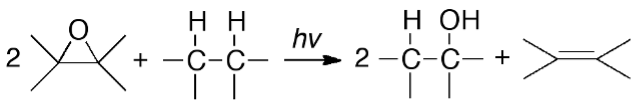
\includegraphics[width=80mm]{figures/fig_equation1.png}
    \label{fig:equation1}
\end{figure}

また,エポキシ基が吸着水と反応して,ヒドロキシ基を形成する過程も存在する.

\begin{figure}[H]
    \centering
    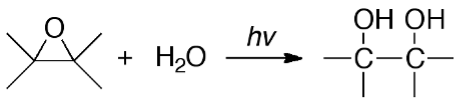
\includegraphics[width=60mm]{figures/fig_equation2.png}
    \label{fig:equation2}
\end{figure}

上記の反応では酸素原子は除去されていないが,これは酸素の除去がヒドロキシ基やカルボニル基の解離によるものと推測される.
例えば,ヒドロキシ基ではVUV光によって励起されると,下式のようにヒドロキシルラジカル,H$_2$O, O, O$_2$が放出され,残存する炭素ラジカルが互いに反応し,C=CもしくはC-Cを形成する\supercite{smirnov_photochemical_2013}.

\begin{figure}[H]
    \centering
    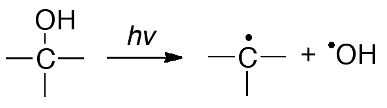
\includegraphics[width=50mm]{figures/fig_equation3.png}
    \label{fig:equation3}
\end{figure}

\begin{figure}[H]
    \centering
    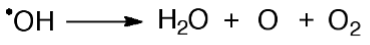
\includegraphics[width=45mm]{figures/fig_equation4.png}
    \label{fig:equation4}
\end{figure}

\begin{figure}[H]
    \centering
    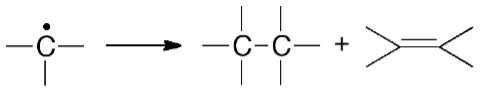
\includegraphics[width=60mm]{figures/fig_equation5.png}
    \label{fig:equation5}
\end{figure}

rCGO\_140ではrGOと比較して,さらに酸素原子が除去されていることがTable\ref{tab:xps}からわかった.
これは,GO表面の吸着水がVUV光によって励起され,Gシート内の炭素原子をエッチングするのを加熱処理が防ぐためと推測される.

\indent
Kha Tuらは,GOを熱還元した際に286.7 eVのピークが消失せず,ある程度のOFGが残存していることを報告している\supercite{tu_remarkable_2015}.
彼らは286.7 eVのピークがヒドロキシ基,エーテル,エポキシ基で構成されているC-O結合に由来するとし,還元後も残存していたピークがエッジ部のsp$^2$結合のC-O-C(エーテル)に起因していると推測している.
本実験では,Kha Tuらの条件とは異なり,286.2 eVにC-OH,286.9 eVにC-O-Cを割り当てているが,今回の結果からエッジ部にsp$^2$結合のC-O-C(エーテル)が存在する可能性があることがわかった.

\begin{figure}[H]
    \centering
    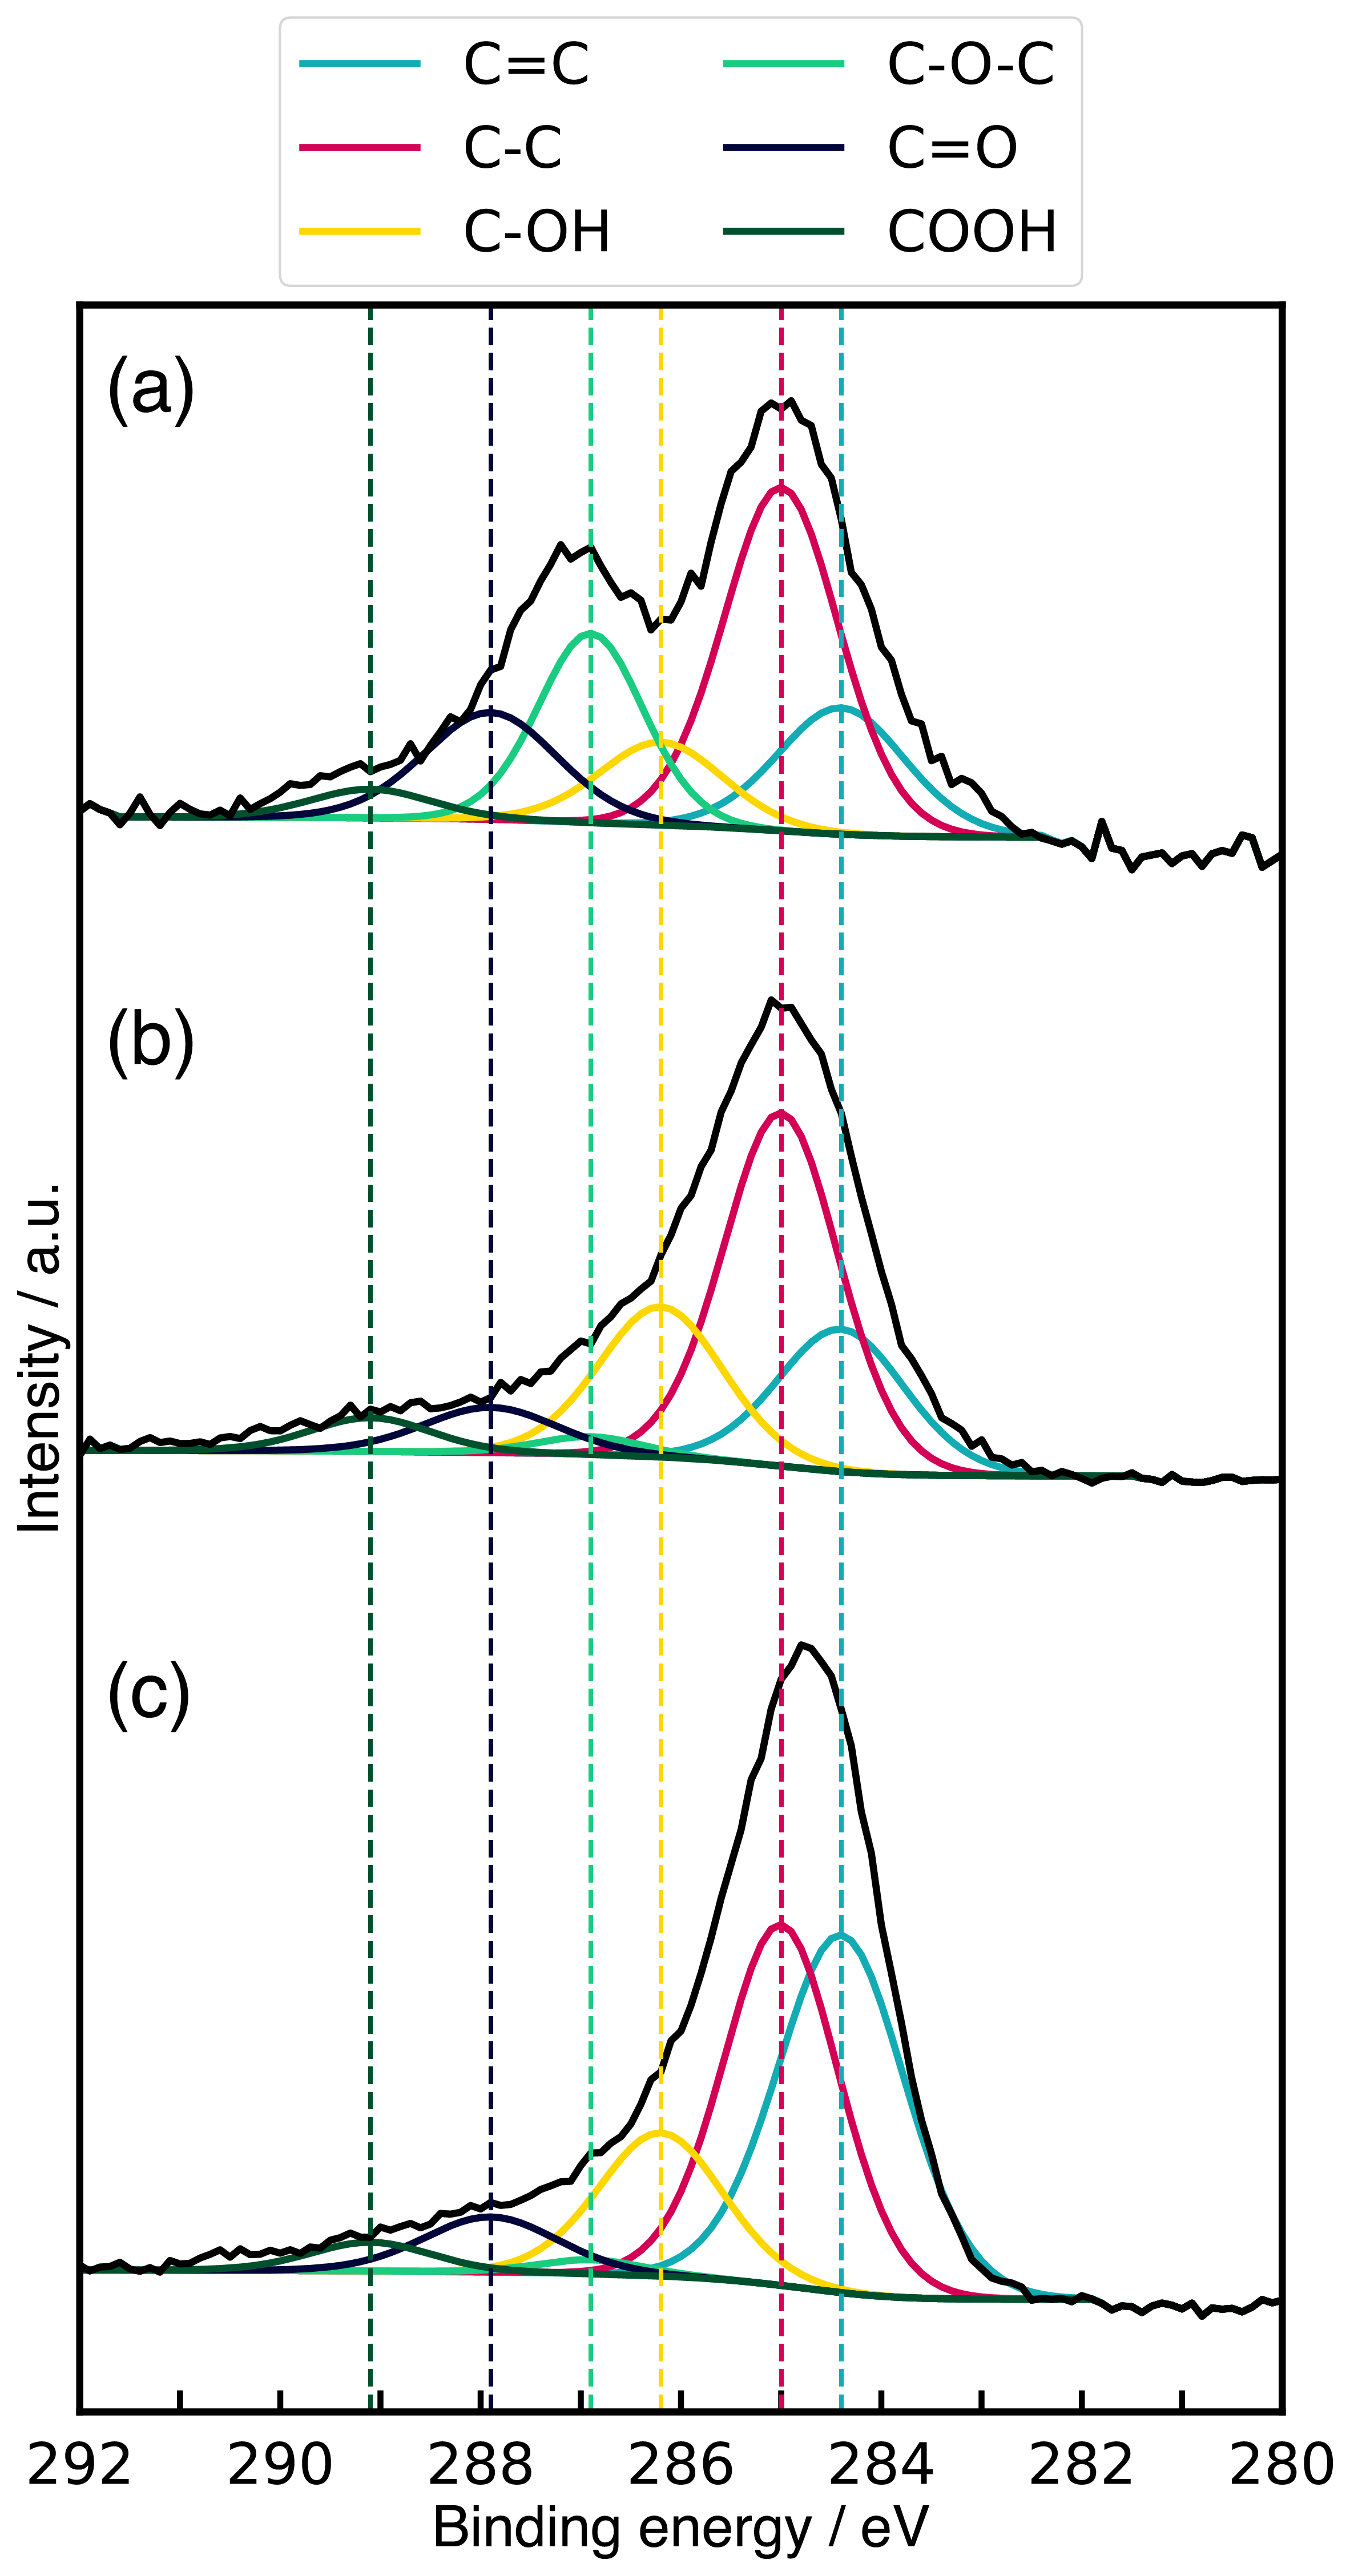
\includegraphics[width=60mm]{figures/figure3.png}
    \caption{XPS C 1s spectra of (a) GO, (b) rGO, (c) rGO\_140.}
    \label{fig:XPS}
\end{figure}

\subsubsection*{\ul{micro Raman spectroscopy}}
Fig.\ref{fig:Raman}は各GOのラマンスペクトルを示す ((a) GO, (b) rGO, (c) rGO\_140).
1340 cm$^{-1}$付近のピークはDピーク,1574 cm$^{-1}$付近のピークはGピークと呼ばれている.
Dピークは逆空間Brillouin zoneのK点でのA$_{\mathrm{1g}}$ breathingモードによる一次散乱である\supercite{ferrari_raman_2013}.
Dピークはグラフェン結晶中のエッジやsp$^3$炭素などの欠陥により六員環の対称性が乱れることで活性化する.
これに対して,Gピークは逆空間Brillouin zoneの$\Gamma$点でのE$_{\mathrm{2g}}$ フォノンによる一次散乱である.
すなわち,sp$^2$炭素ペアの伸張に起因している.
1620 cm$^{-1}$には欠陥によって誘発されるもう一つのピークが存在し,これはD'ピークと呼ばれている.
スコッチテープから剥離して得られた(多層)グラフェンでは,Gピークが1574 cm$^{-1}$付近に現れていることがわかった(破線) (Fig.\ref{fig:Raman} (a)).
また,DピークがGピークに対して極めて弱く,グラフェン中には欠陥が少ないことが示唆された.
一方,GOのスペクトルでは,Dピークが1340 cm$^{-1}$付近に顕著に現れ,そしてGピークが高波数側である1604 cm$^{-1}$にシフトしていた(破線ドット).
このGピークはGとD'の混合ピークであると上記の議論から推測できる.
これらの結果から,化学剥離によって作製したGO\supercite{hirata_thin-film_2004}では,OFGやsp$^3$-Cなどの欠陥が導入され,ハニカム構造が破壊されたことがわかった.\\
\indent
rGO,rGO\_140では,VUV光還元によってGピークが1604 cm$^{-1}$から1594 cm$^{-1}$付近へとレッドシフトしていることがわかる 
このシフトはD'ピークに対するGピークの割合の増加を意味しており,VUV照射によって共役結合が再構築されたことが示唆された.

\begin{figure}[H]
    \centering
    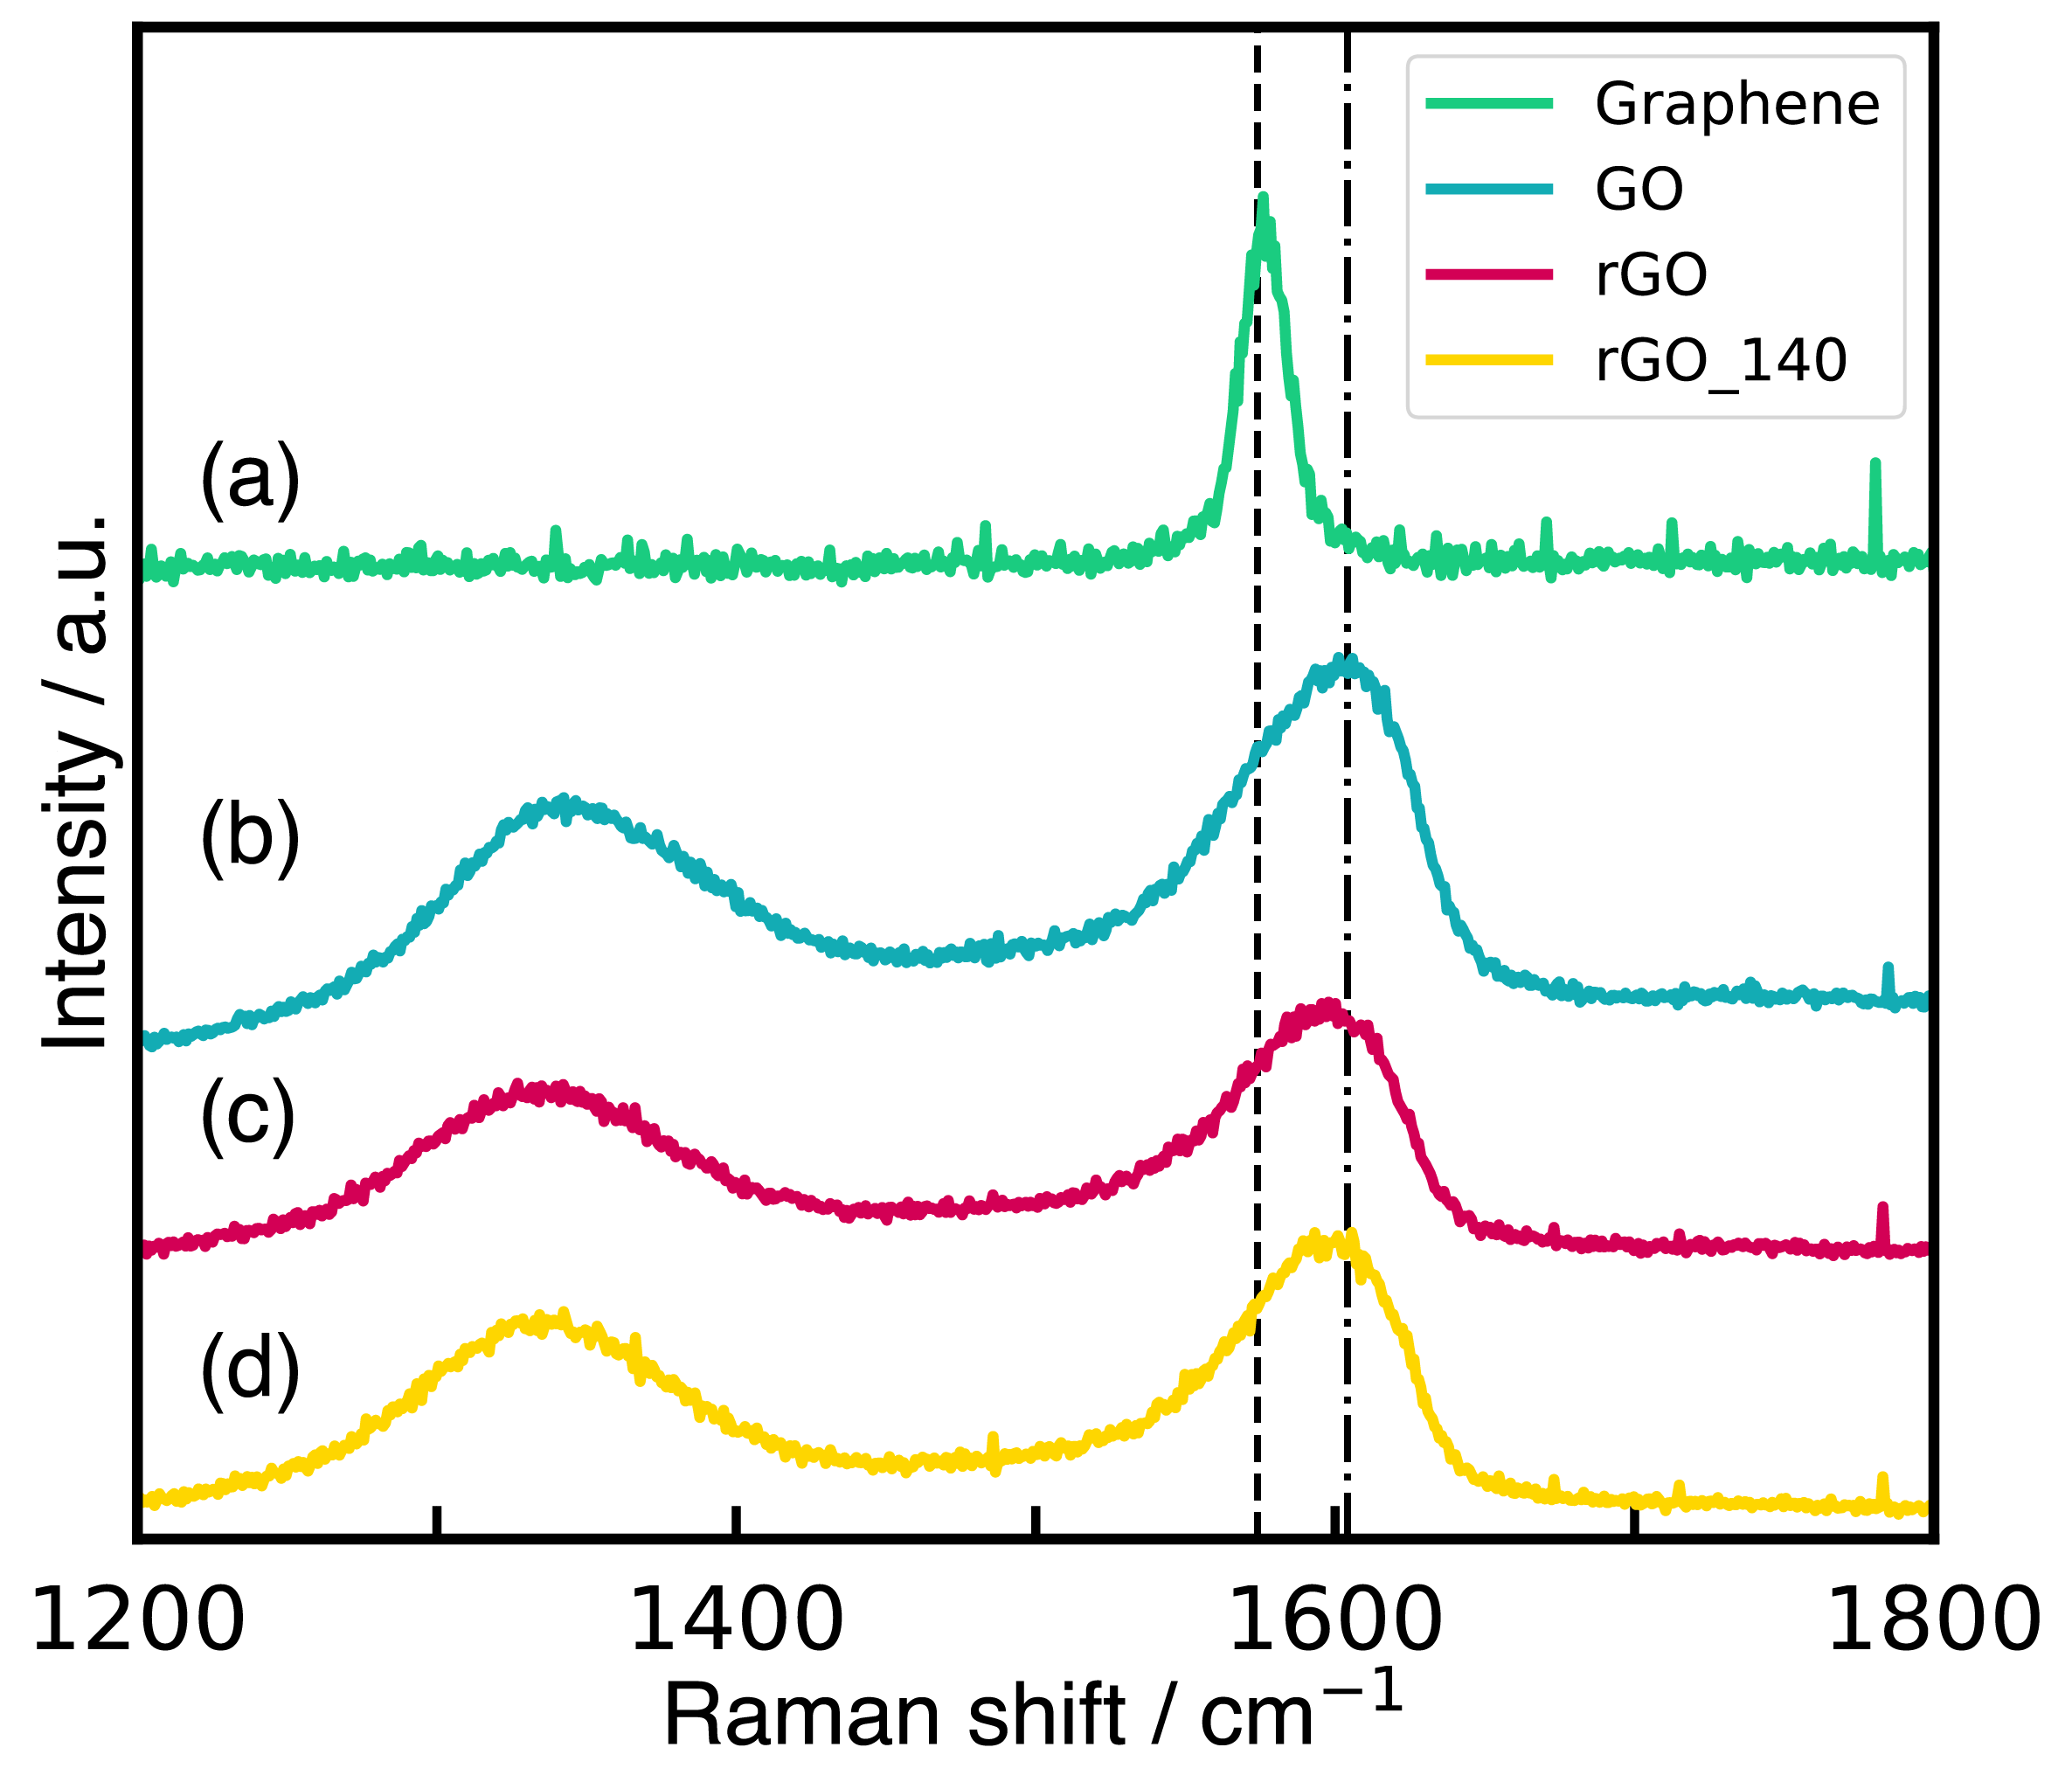
\includegraphics[width=100mm]{figures/figure4.png}
    \caption{Raman spectra of (a) GO, (b) rGO, (c) rGO\_140.}
    \label{fig:Raman}
\end{figure}

\subsubsection*{\ul{Conclusion}}
化学剥離法およびVUV光照射を用いることで,シート面内の構造の異なるGOを作製することが可能であることが明らかとなった.
また,VUV光照射によってGOの電気伝導度が向上したという報告もあり,光照射がGOの還元,すなわちsp$^2$ドメインを修復するのに有用であることが明らかとなった.

\newpage
\section*{\ul{Experiment 2. Vapor etching of GO/rGO-coated silicon}}

\subsection*{\ul{Purpose of this experiment}}
上記のGO,rGO,rGO\_140を用いてエッチングを行うことでGOシート面内の構造がエッチング挙動に与える影響を明らかにする.
そして,GOアシストシリコンエッチング反応の律速過程を同定することで,エッチング速度の高速化や,高アスペクト比の達成の実現を目標とする.
本研究で作製したGOはシート毎に微視的な構造が異なるだけでなく,そのサイズが不均一である(Fig.\ref{fig:AFM}).
窪田らはGOシートのサイズが小さいほどエッチング速度が向上するという結果を示しているため\supercite{kubota_vapor-phase_2022},本実験ではシートサイズのバラつきを解消しなければならない.
また、単なるスピンコーティングでは,基板上のGOが不均一に分布し,凝集体を形成する可能性があるため,位置の制御が望ましい.
そこで,本実験では,マイクロコンタクトプリンティング (Microcontact Printing: \textmu CP)と呼ばれるパターニング手法を用いて\supercite{xiao_micro-contact_2014},GOシートのサイズおよび位置制御を行い,画一的にエッチング挙動について評価する.
\textmu CPではシクロオレフィンポリマー (Cyclo Olefin Polymer: COP)を用いる (Fig.\ref{fig:COP} (a)).
COPはその表面にVUV光を照射することで,大気中の励起した活性酸素種との反応により,疎水性から親水性へと表面改質が進行するだけでなく,エッチング反応が進行する\supercite{sugimura_vacuum_2012}.
このCOPフィルムをスタンプとして利用することで,簡易的な\textmu CPを試みる.

\subsection*{\ul{Experimental procedure}}
\begin{enumerate}
    \item 2 $\times$ 2 cm$^2$ Si (boron-doped p-type (100), 1 - 30 $\Omega\cdot$cm) substrates or Si substrates covered with a thermal oxide layer (boron-doped p-type (100), 90 nm SiO$_2$, 0.1 $\Omega\cdot$cm) were ultrasonically cleaned by acetone, ethanol, and UPW for 30 min respectively and then cleaned by VUV (Xe) light irradiation for 20 min.
    \item Cyclo Olefin Polymer (COP) films (ZF14-188, ZeonorFilm, Zeon Inc.) were cut into 2 $\times$ 2 cm$^2$ (Fig.\ref{fig:COP} (a)).
    \item COP films were irradiated by VUV light via a photomask under 10$^3$ Pa dry air environment for 30 min to form a circle-pattern with a diameter 10 \textmu m. 
    \item GO dispersion was pulverized for 6 hours to uniform the sheet sizes of GO to less than some \textmu m.
    \item The GO dispersion was deposited onto the COP film by spin-coating (500 rpm for 15 s and then 2000 rpm for 150 s).
    \item The COP film with GO was pushed against the cleaned silicon or silicon dioxide substrate with a load of 400 N for 1 h to transfer the GO circle pattern on the substrate. (These processes are shown in Fig.\ref{fig:COP} (b))
    \item The PFA container for etching was washed with acetone (sonicated for 30 min), a solution containing dil. HCl (heated at 80 ${}^\circ$C for more than 30 min), and UPW (sonicated for 30 min).
    \item The small PFA cpntainer with the etchant which is the mixture of HF 5 mL (50 wt\%, for the semiconductor industry, Morita Chemical Industry Corp.) and H$_2$O$_2$ 100 \textmu L (30 wt\%, analytical grade, Fuji Film Wako Pure Chemical Corp.) was sealed in the large PFA container, and heated at 60 ${}^\circ$C for longer than 90 min so that the etchant temperature remained at 50 ${}^\circ$C.
    \item The silicon substrate with the circle patterning of GO, rGO, or rGO\_140 was sealed in the PFA container and kept at 60 ${}^\circ$C for 16 h.
    \item After etching, the surface of the silicon substrate was observed by 3D-Laser microscope.
    \item Additionally, the substrate was cleaved and washed with UPW to observe the surface and cross-section by Field Emission-type Scannig Electron Microscope (FE-SEM).
\end{enumerate}

\begin{figure}[H]
    \centering
    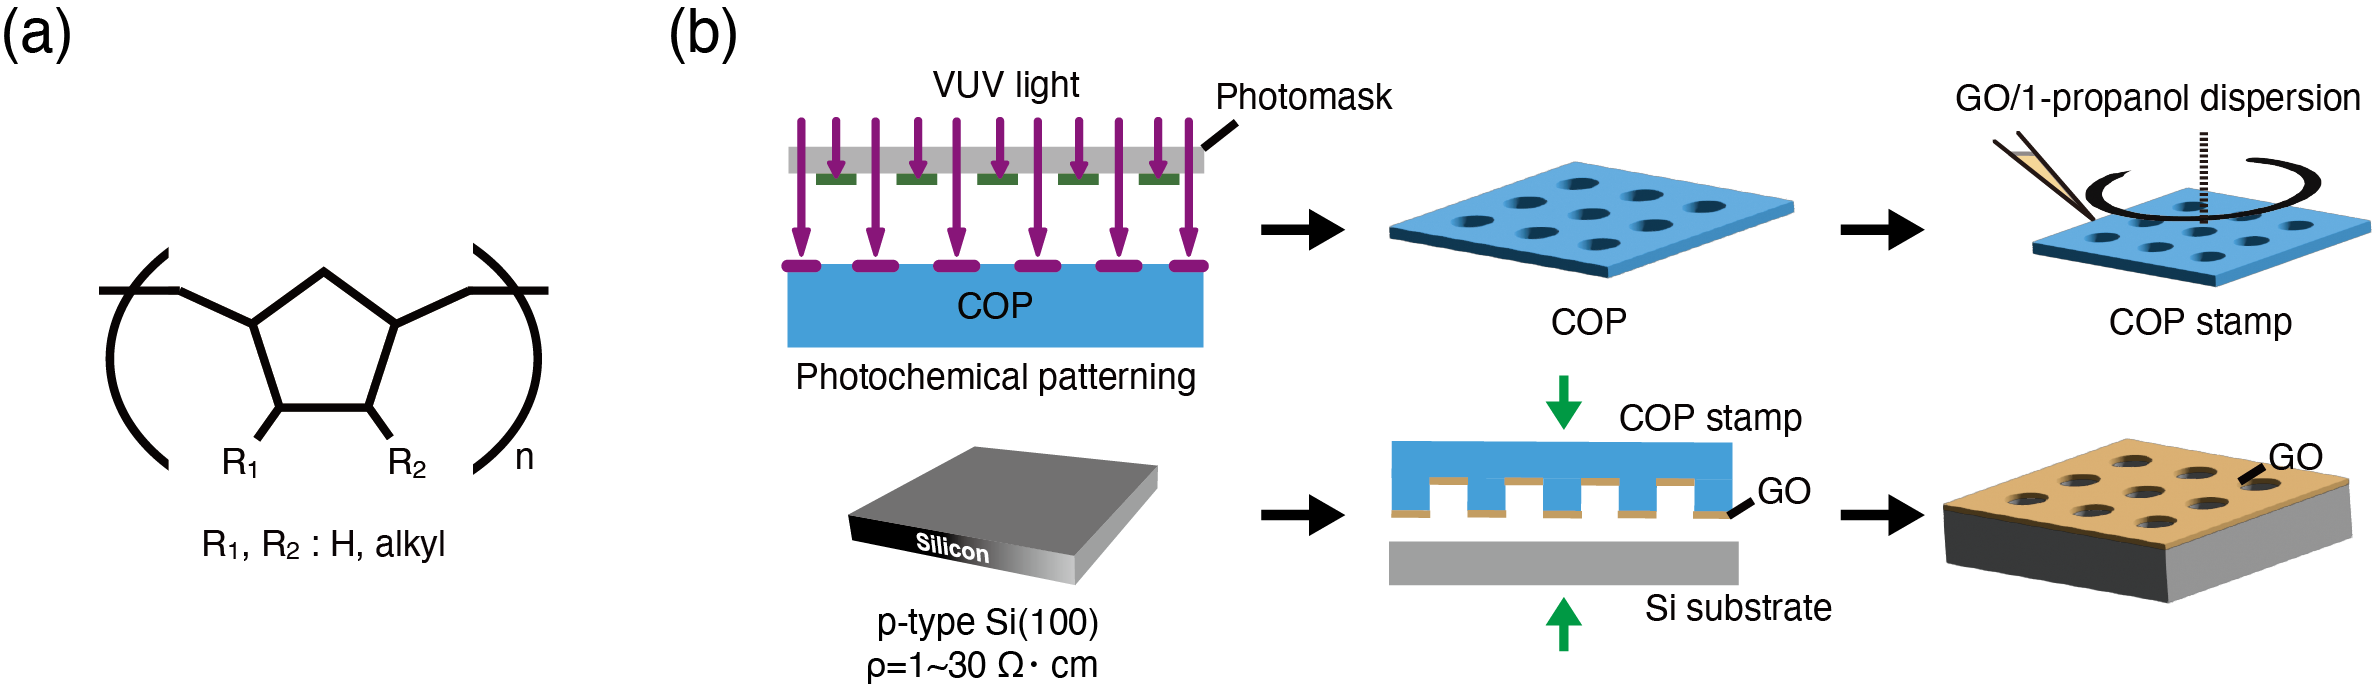
\includegraphics[width=120mm]{figures/figure5.png}
    \caption{(a) An image of the chemical structure of COP and (b) a schematic illustration of the microcontact patterning process using COP films.}
    \label{fig:COP}
\end{figure}

\subsection*{\ul{Results and discussion}}

Fig.\ref{fig:COP_AFM}(a)は,VUV光照射後のCOPフィルムのAFM像を示している.
VUV光によって,COPフィルムの照射部がフォトマスクの円形パターンと同じ幅でエッチングされていることがわかる.
このエッチング反応は2段階の反応に分けられる\supercite{sugimura_ultra-violet_2018}.
まず,COPフィルムの表面が活性酸素種により酸化され,カルボン酸やカルボニル基,ヒドロキシ基が生成される.
そして,表面の酸化層がCO$_2$,CO,H$_2$Oまで酸化され,揮発脱離,すなわちエッチングが進行する.
Fig.\ref{fig:COP_AFM}(b), (c)は,VUV光照射後のCOPフィルム上にGOをスピンコートしたのちにSiO$_2$上にスタンプした後のAFM像である.
スタンプ後も直径が10 \textmu mの円形パターンが形成されていることもあれば (Fig.\ref{fig:COP_AFM}(b)),Fig.\ref{fig:COP_AFM}(c)のように円形が崩れ,直径が10 \textmu mよりも大きなパターンが得られることもあった.
これはCOPフィルム上にGO分散液をスピンコーティングする際に,GOが均一にCOP上に分散していなかった,もしくはスタンプ中にSiO$_2$へのGOの転写が適切に行われなかったことが考えられる.
SiO$_2$上に転写されたGOの高さは平均して数 nmとなっており単層(およそ1 nm),もしくは数層重なったGOが混在して存在していることが明らかになった.

\begin{figure}[H]
    \centering
    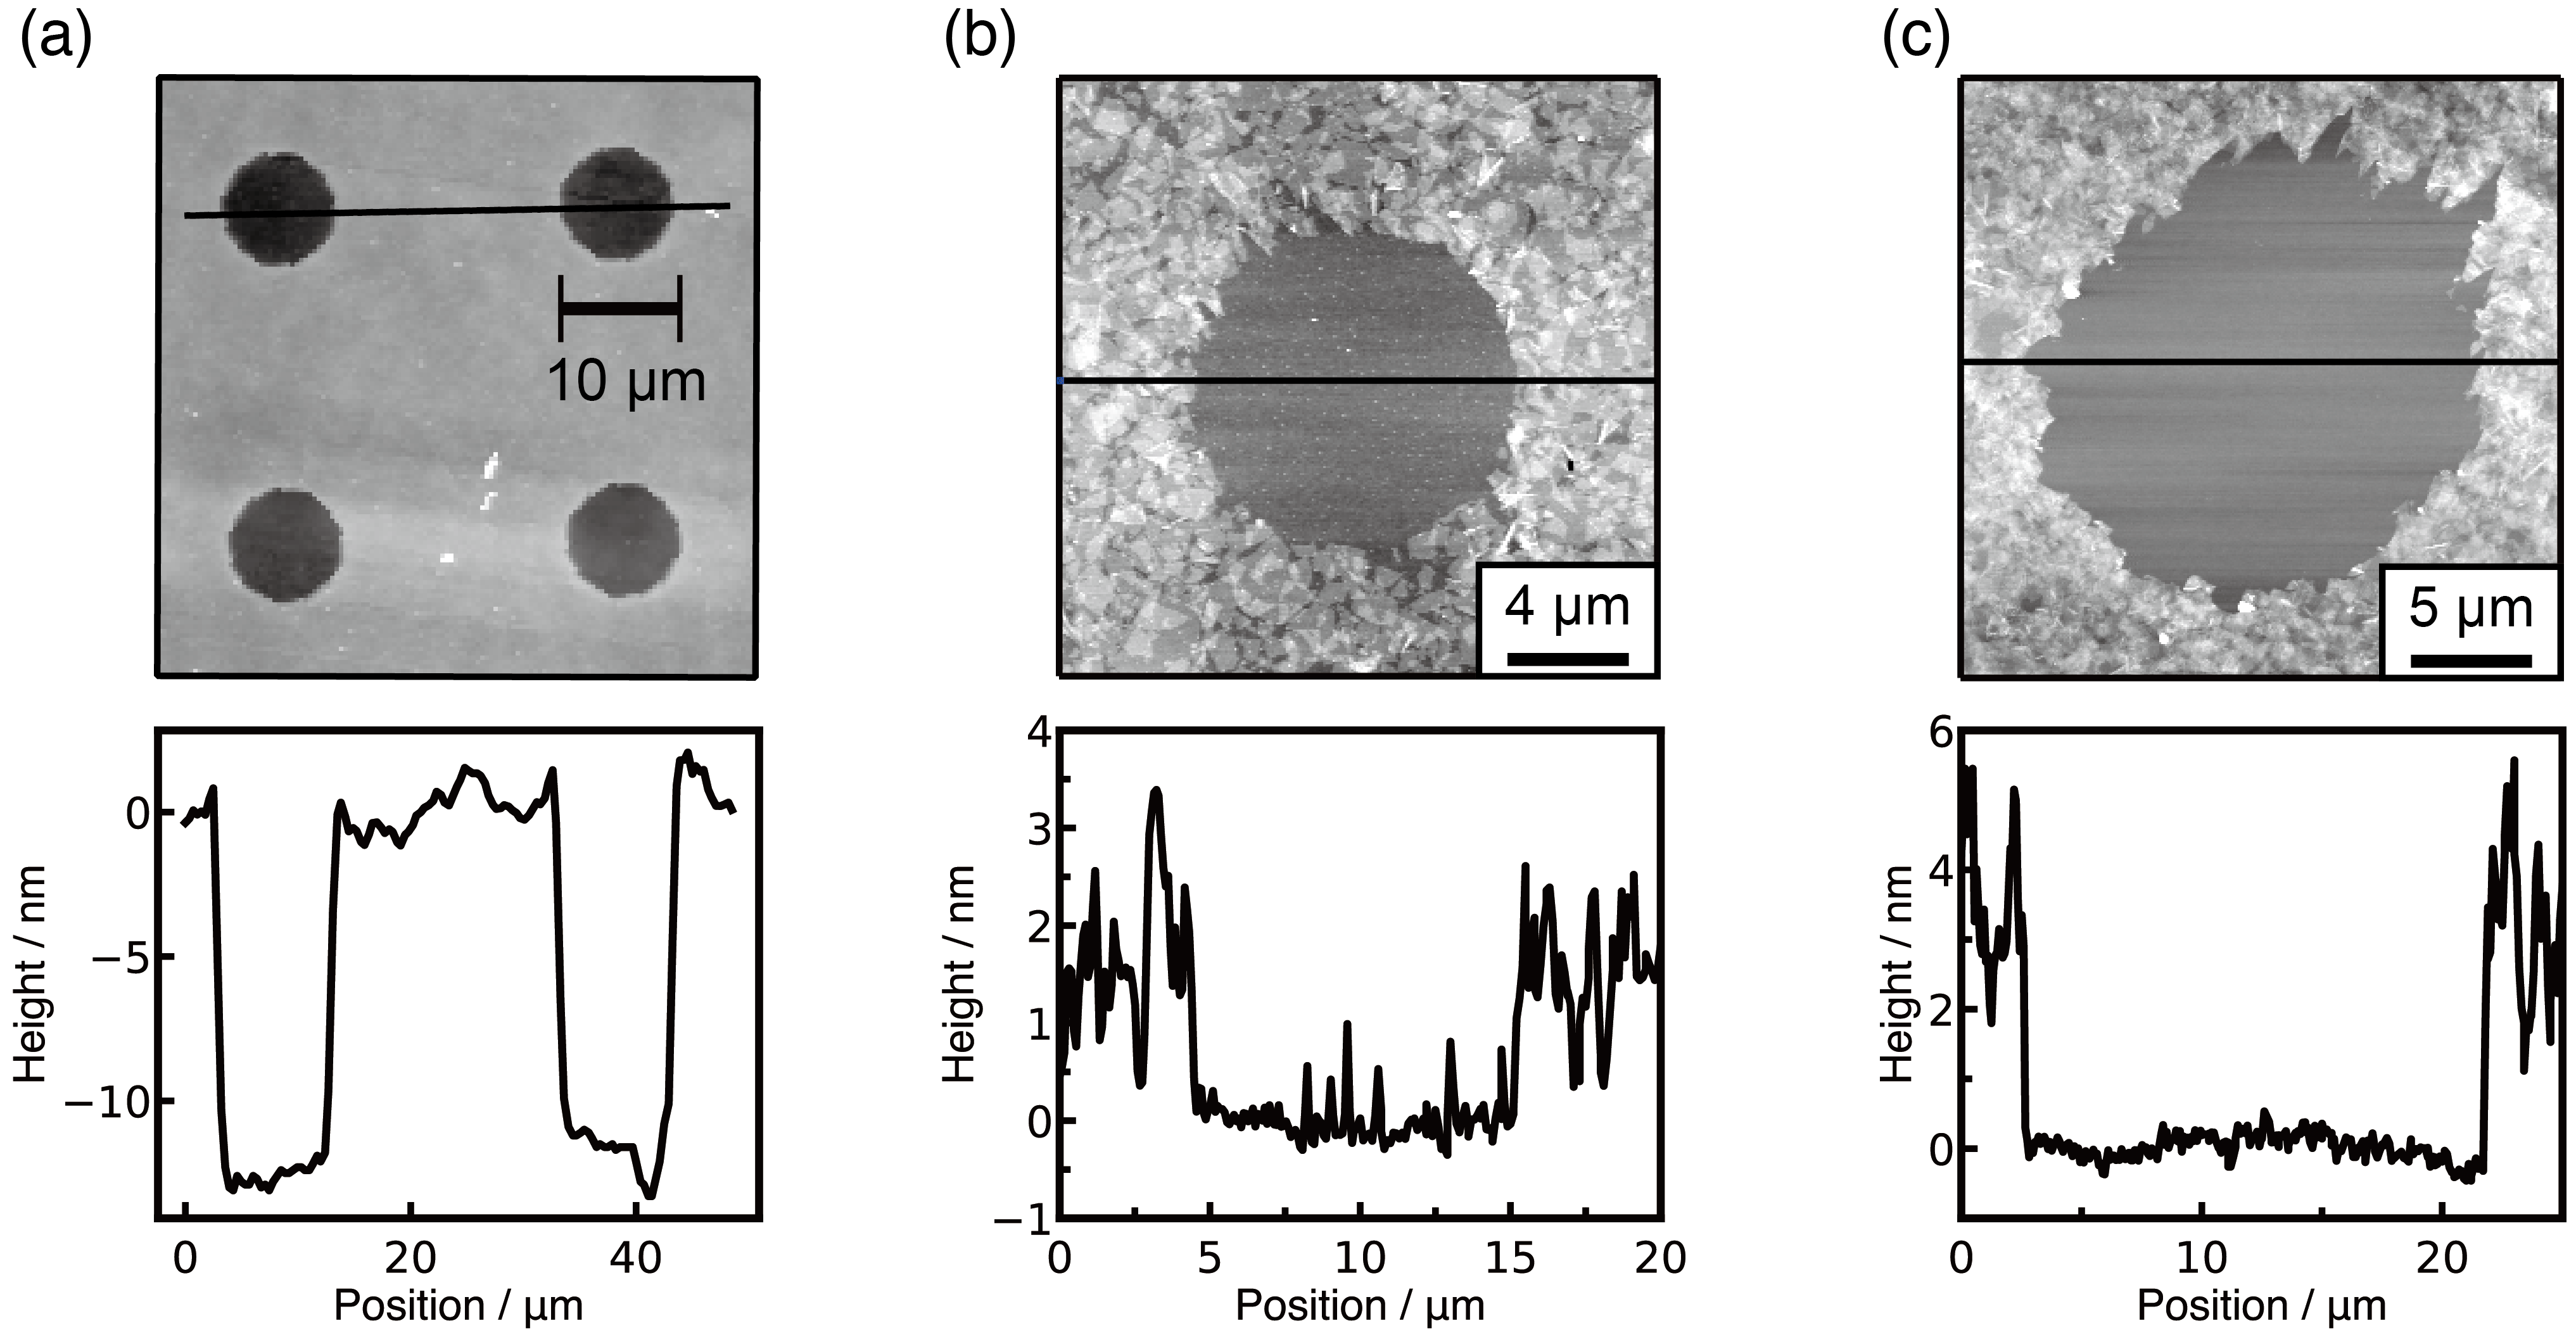
\includegraphics[width=150mm]{figures/figure6.png}
    \caption{AFM topographic images and cross-sectional profiles along the lines of (a) a COP film after VUV light irradiation, (b) and (c) patterned GO sheets on a SiO$_2$ substrate.}
    \label{fig:COP_AFM}
\end{figure}

次に,フッ酸と過酸化水素からなるエッチャントを50 ${}^\circ$Cに加熱し,その蒸気をスタンプ後のGO担持シリコンに16時間,暴露させた.
ここで用いたエッチャントの組成は[HF] = 29 mol/L, [H$_2$O$_2$] = 0.2 mol/Lである.
Fig.\ref{fig:Laser}(a),(b),(c)はそれぞれ,(a) GO, (b) rGO, (c) rGO\_140を担持したシリコンのエッチング後の高さプロファイルを示している.
どの試料でもエッチングによって形成された凹凸の深さはおよそ300 nmから 500 nmであった.
フッ酸によるシリコンの溶解反応は次式で表される\supercite{fukuta_vapor_2003, hildreth_vapor_2014}.
\begin{displaymath}
    \mathrm{Si + 4HF + 4h^+ \rightarrow SiF_4 + 4H^+}
\end{displaymath}
ここで,GOは酸化剤(H$_2$O$_2$)還元反応を促進し,シリコン表面の正孔濃度を増加させるため,GOに覆われていないシリコン部分(以降,ベアシリコンと呼ぶ)よりもシリコンの溶解反応が進行する\supercite{kubota_chemical_2019}.
酸化剤還元反応は,
\begin{displaymath}
    \mathrm{H_2O_2 + 2H^+ + 2e^- \rightarrow 2H_2O}
\end{displaymath}
である.

Fig.\ref{fig:Laser}(d)はGO,rGO,rGO\_140をそれぞれ用いて16時間,50 ${}^\circ$Cでエッチングを行った際に形成された凹凸の深さをまとめたものである.
丸印は平均の深さを表しており,GOで約450 nm,rGOで約400 nm,そしてrGO\_140で約500 nmとなった.
rGOやrGO\_140ではGOと比較して構造欠陥が修復されており,酸化剤還元によってシリコンに注入できる成功濃度も異なると推測される.
実際に,液相において,従来の化学剥離法で作製されたGOと電気化学剥離法によって作製された構造欠陥の少ないGO (Electrichemically exfoliated Graphene Oxide: EGO)を用いたエッチングでは,EGOを担持したシリコンの方がエッチング速度が遅いという結果が示されている\supercite{kubota_chemical_2021}.
それにも拘らず,各試料間でのエッチング速度の顕著な差は確認されなかった.
したがって,GOを用いたシリコン気相エッチングでは,GOとシリコン間において生成物が反応物(HF)の拡散を阻害していると推測した.

\begin{figure}[H]
    \centering
    \includegraphics[width=165mm]{figures/figure7.png}
    \caption{3D laser microscopic topographic images and cross-sectional profiles along the black lines of etched silicon with (a) GO, (b) rGO, (c) rGO\_140 at 50 ${}^\circ$C for 16 h. The relationship between the samples and the etching depth at 50 ${}^\circ$C for 16 h is shown in (d).}
    \label{fig:Laser}
\end{figure}

ここで,HFが律速反応の場合,シリコンの溶解反応は以下のようになる\supercite{fukami_roles_2018}.
\begin{displaymath}
    \mathrm{Si + 2H_2O+ 4h^+ \rightarrow SiO_2 + 4H^+}
\end{displaymath}
\begin{displaymath}
    \mathrm{SiO_2 + 4HF \rightarrow SiF_4 + 2H_2O}
\end{displaymath}
この時,XPSによってSiO$_2$の存在を確認することができるとされている.
しかし,窪田らの報告によると,エッチング後の試料におけるXPSでは,103.5 eV付近にピークの存在を確認できていない\supercite{kubota_vapor-phase_2022}.
つまり,気相エッチングでは,HFの拡散が律速過程ではないことが明らかとなった.

ここで,さらにその律速過程を同定するために,(i)酸化剤濃度を増加,もしくは(ii)エッチング温度を増加させてエッチングを行うことにした.
H$_2$O$_2$の濃度を0.2 mol/Lから0.4 mol/Lに増加してGOを担持したシリコンをエッチングした後の高さプロファイルを示している.

\begin{figure}[H]
    \centering
    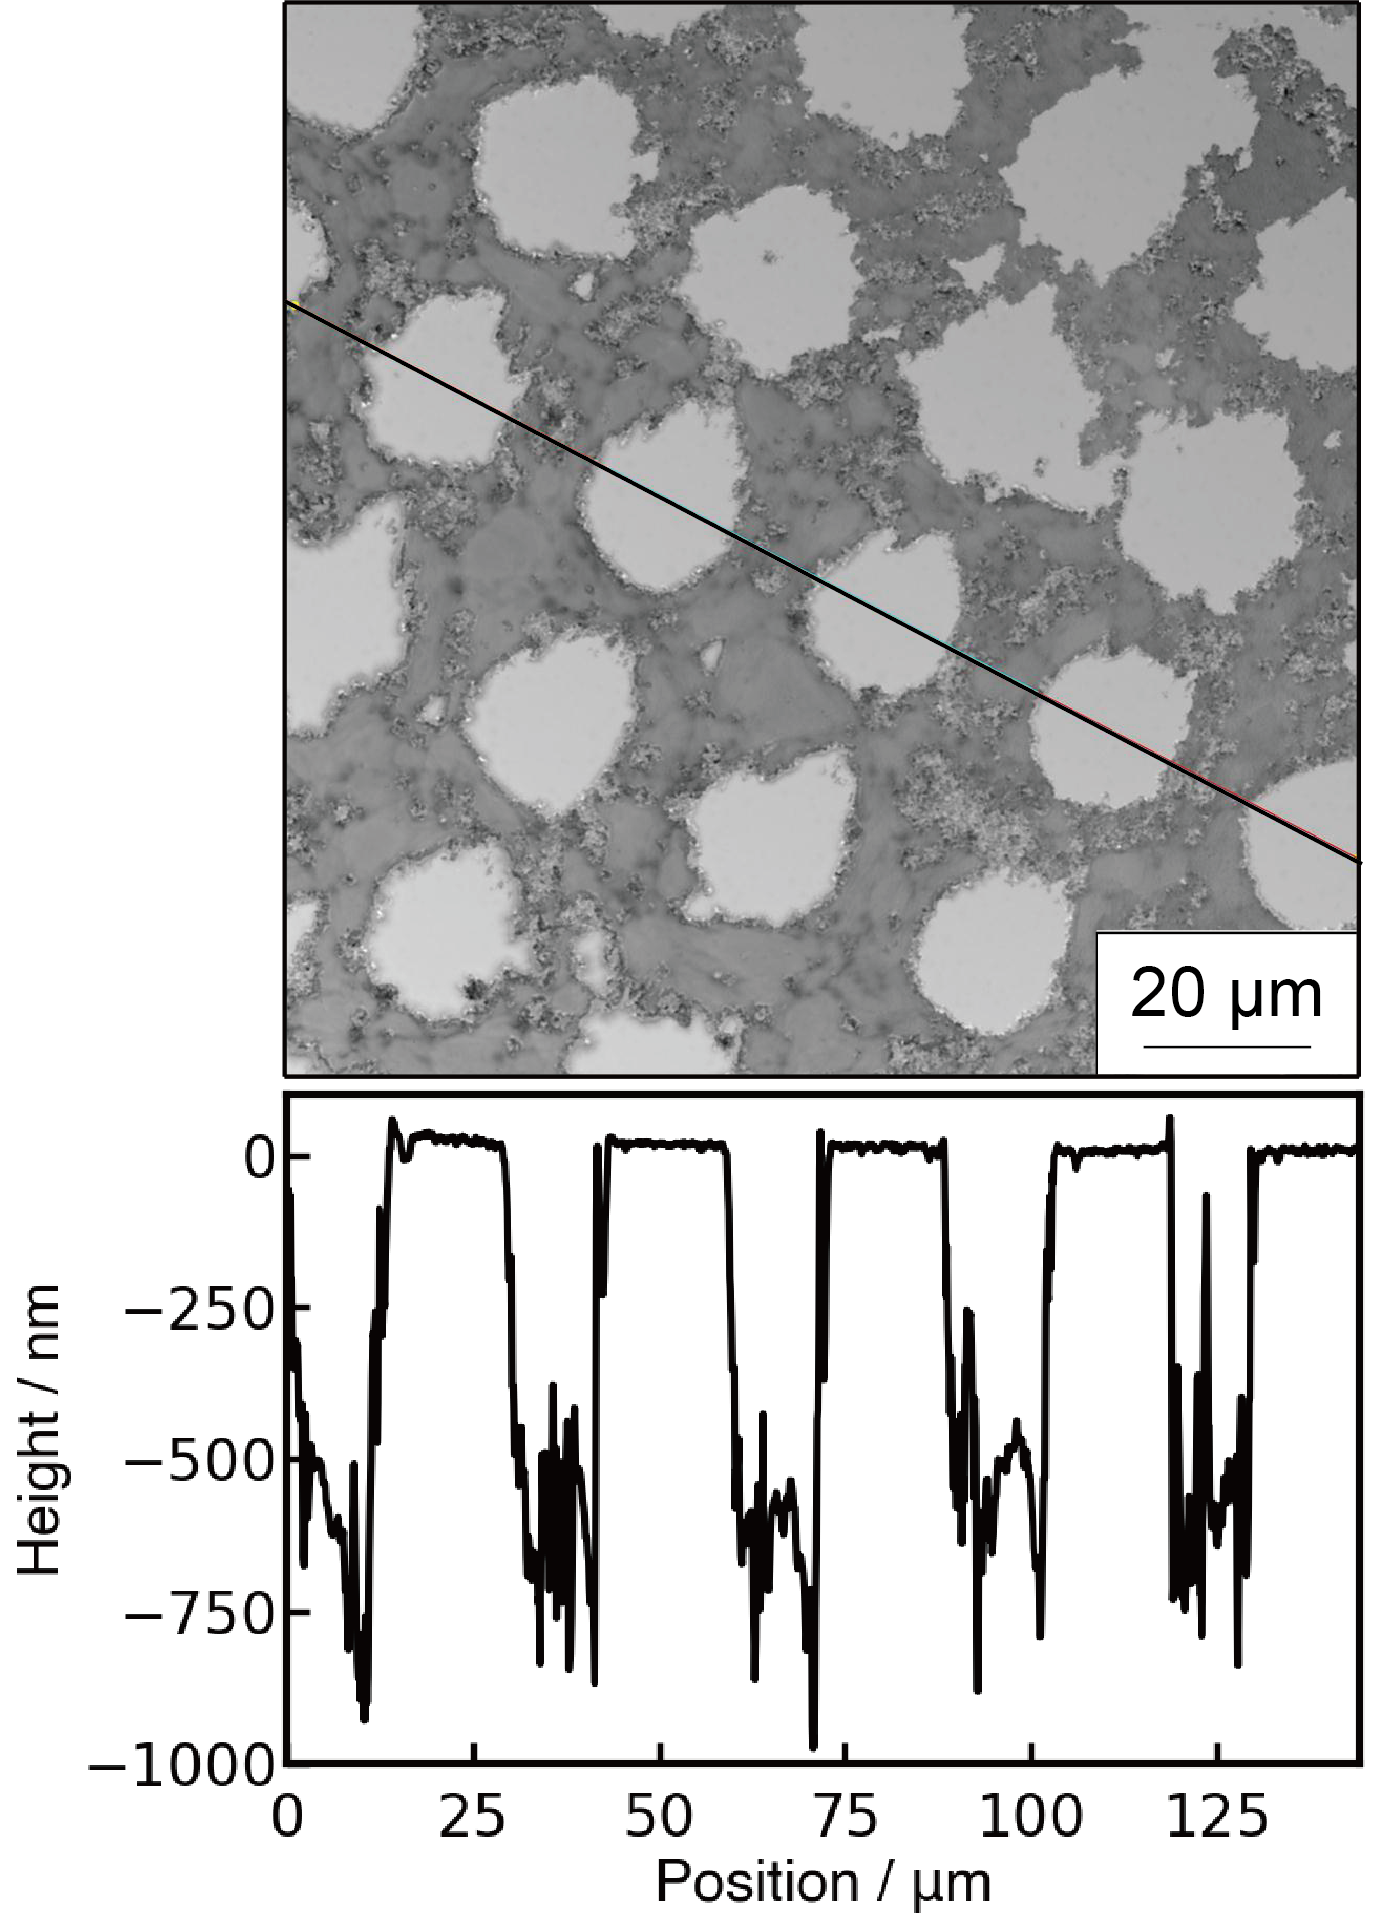
\includegraphics[width=70mm]{figures/figure11.png}
    \caption{A 3D laser microscopic topographic images and cross-sectional profiles along the black line of etched silicon with GO at 50  ${}^\circ$C for 16 h.}
    \label{fig:Laser_h2o2}
\end{figure}

酸化剤濃度を2倍にするとエッチング深さは平均で約600 nmとなっており,増加していた.
酸化剤濃度をさらに上げた際のエッチング挙動について確認する必要があるが,以上の結果から反応律速であることが示された.
すなわち,GOが酸化剤還元を促進するのは欠陥の中でも,VUV光還元によって修復されないエッジや空孔といった欠陥であり,sp$^2$ドメインやOFGなどはエッチング反応にわずかな寄与しか有さないと推測される.
Denisらはグラフェン上の欠陥と官能基の結合エネルギーを第一原理計算によって導出しており,基本的には反応性は単一空孔,エッジ,欠陥のないグラフェンの順に低くなると述べている\supercite{denis_comparative_2013}.
しかし,島川らは液相でのエッチングではrGOがマスクとして機能し,エッチング反応を阻害していたと述べており(島川修論),液相と気相でGOの酸化剤との反応のメカニズムが異なることも示唆される結果となった.

次に,温度と各試料のエッチング挙動の関係について調べた.
Fig.\ref{fig:Etching_temp}(a)はエッチング温度が60 ${}^\circ$Cの時の凹凸の深さプロファイルを表しており,それぞれ,(a-1) GO, (a-2) rGO, (a-3) rGO\_140となっている.
Fig.\ref{fig:Etching_temp}(b)も同様にエッチング温度が70 ${}^\circ$Cの時の凹凸の深さプロファイルを表しており,それぞれ,(a-1) GO, (a-2) rGO, (a-3) rGO\_140である.
どの試料の場合でも,温度が増加にするに伴ってエッチング速度がわずかに上昇する傾向にあり,これは律速過程が反応律速であることに矛盾していない.
Fig.\ref{fig:Etching_temp}(c)は各試料における温度とエッチング速度の関係を表したものである.
丸印はそのエッチング温度でのエッチング深さの平均を表している.
50 ${}^\circ$C, 60 ${}^\circ$Cの場合ではどの試料でもエッチング速度はほとんど変わらなかった.
70 ${}^\circ$CではGO,rGO\_140とrGOの間にエッチング速度のわずかな差が見られたものの,これらの結果からVUV光還元により修復可能な構造欠陥がエッチング速度に与える影響は少ないことがわかった.


\begin{figure}[H]
    \centering
    \includegraphics[width=140mm]{figures/figure8.png}
    \caption{3D laser microscopic topographic images and cross-sectional profiles along the black lines of etched silicon with (a-1) GO, (a-2) rGO, (a-3) rGO\_140 at 60 ${}^\circ$C and (b-1) GO, (b-2) rGO, (b-3) rGO\_140 at 70 ${}^\circ$C for 16 h. The relationship between the temperature and the etching depth for the different samples for 16 h is shown in (d).}
    \label{fig:Etching_temp}
\end{figure}

% Fig.\ref{fig:Schematic_mechanism}は以上の結果から導かれたメカニズムに関しての模式図である.
% Macetchでは金属薄膜を触媒として用いたときに薄膜端のシリコンからエッチングが進行するという報告がある.
% これは反応物,特にHFの供給が,金属薄膜中心下のシリコンよりも薄膜端のシリコンの方が容易だからである.
% GOを用いたエッチングでも同様のことが言えると推測できる(Fig.\ref{fig:Schematic_mechanism} (b)).

% \begin{figure}[H]
%     \centering
%     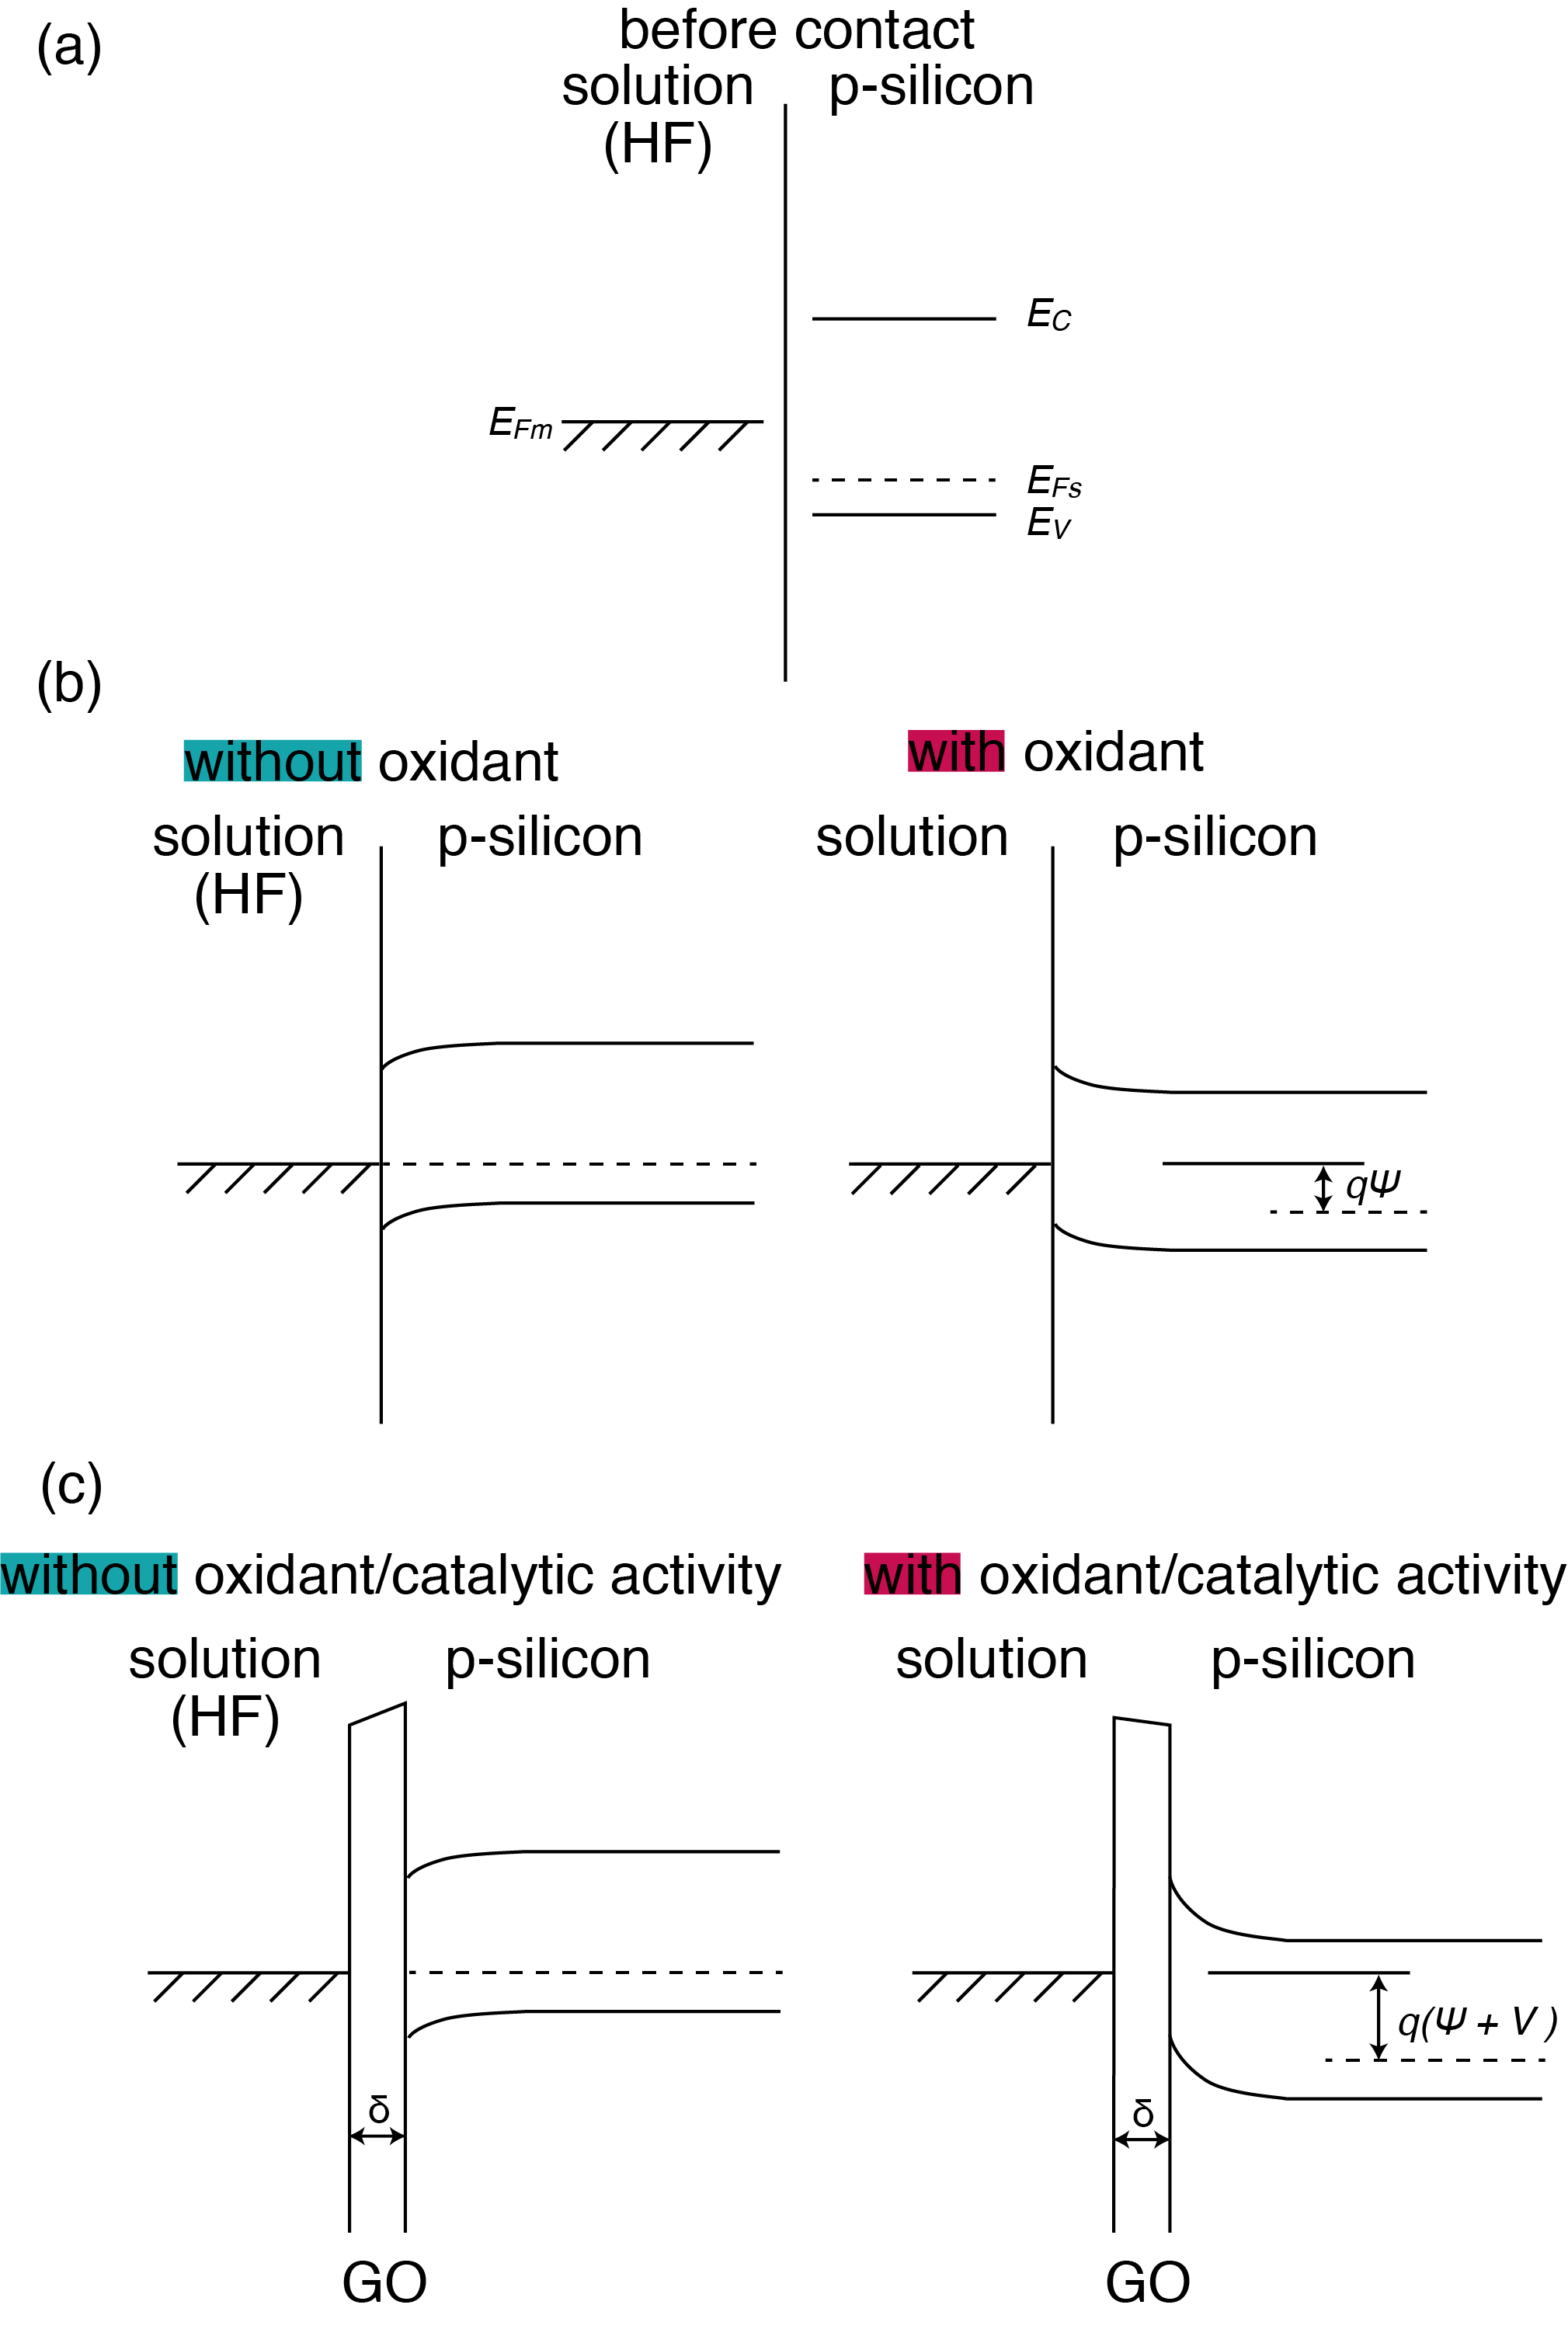
\includegraphics[width=100mm]{figures/appendix1.png}
%     \caption{Schematic illustrations of the mechanism of the vapor-etching with GO.}
%     \label{fig:appendix1}
% \end{figure}

% Fig.\ref{fig:appendix1}はフッ酸と硝酸からなるエッチャントにGOを担持したシリコン基板を4分間浸漬した後の高さプロファイル像である.
% エッジ付近がエッチングされていることがわかる.
% 気相では物質拡散が液相の場合と比較して速いものの,非常に小さなスケールで上記のプロセスが進行していると推測される.\
% \indent
% そして,Siが溶解することで生成物であるSiF$_6^2-$やH$_2$OがSiとGO界面に生じる. 

% \begin{figure}[H]
%     \centering
%     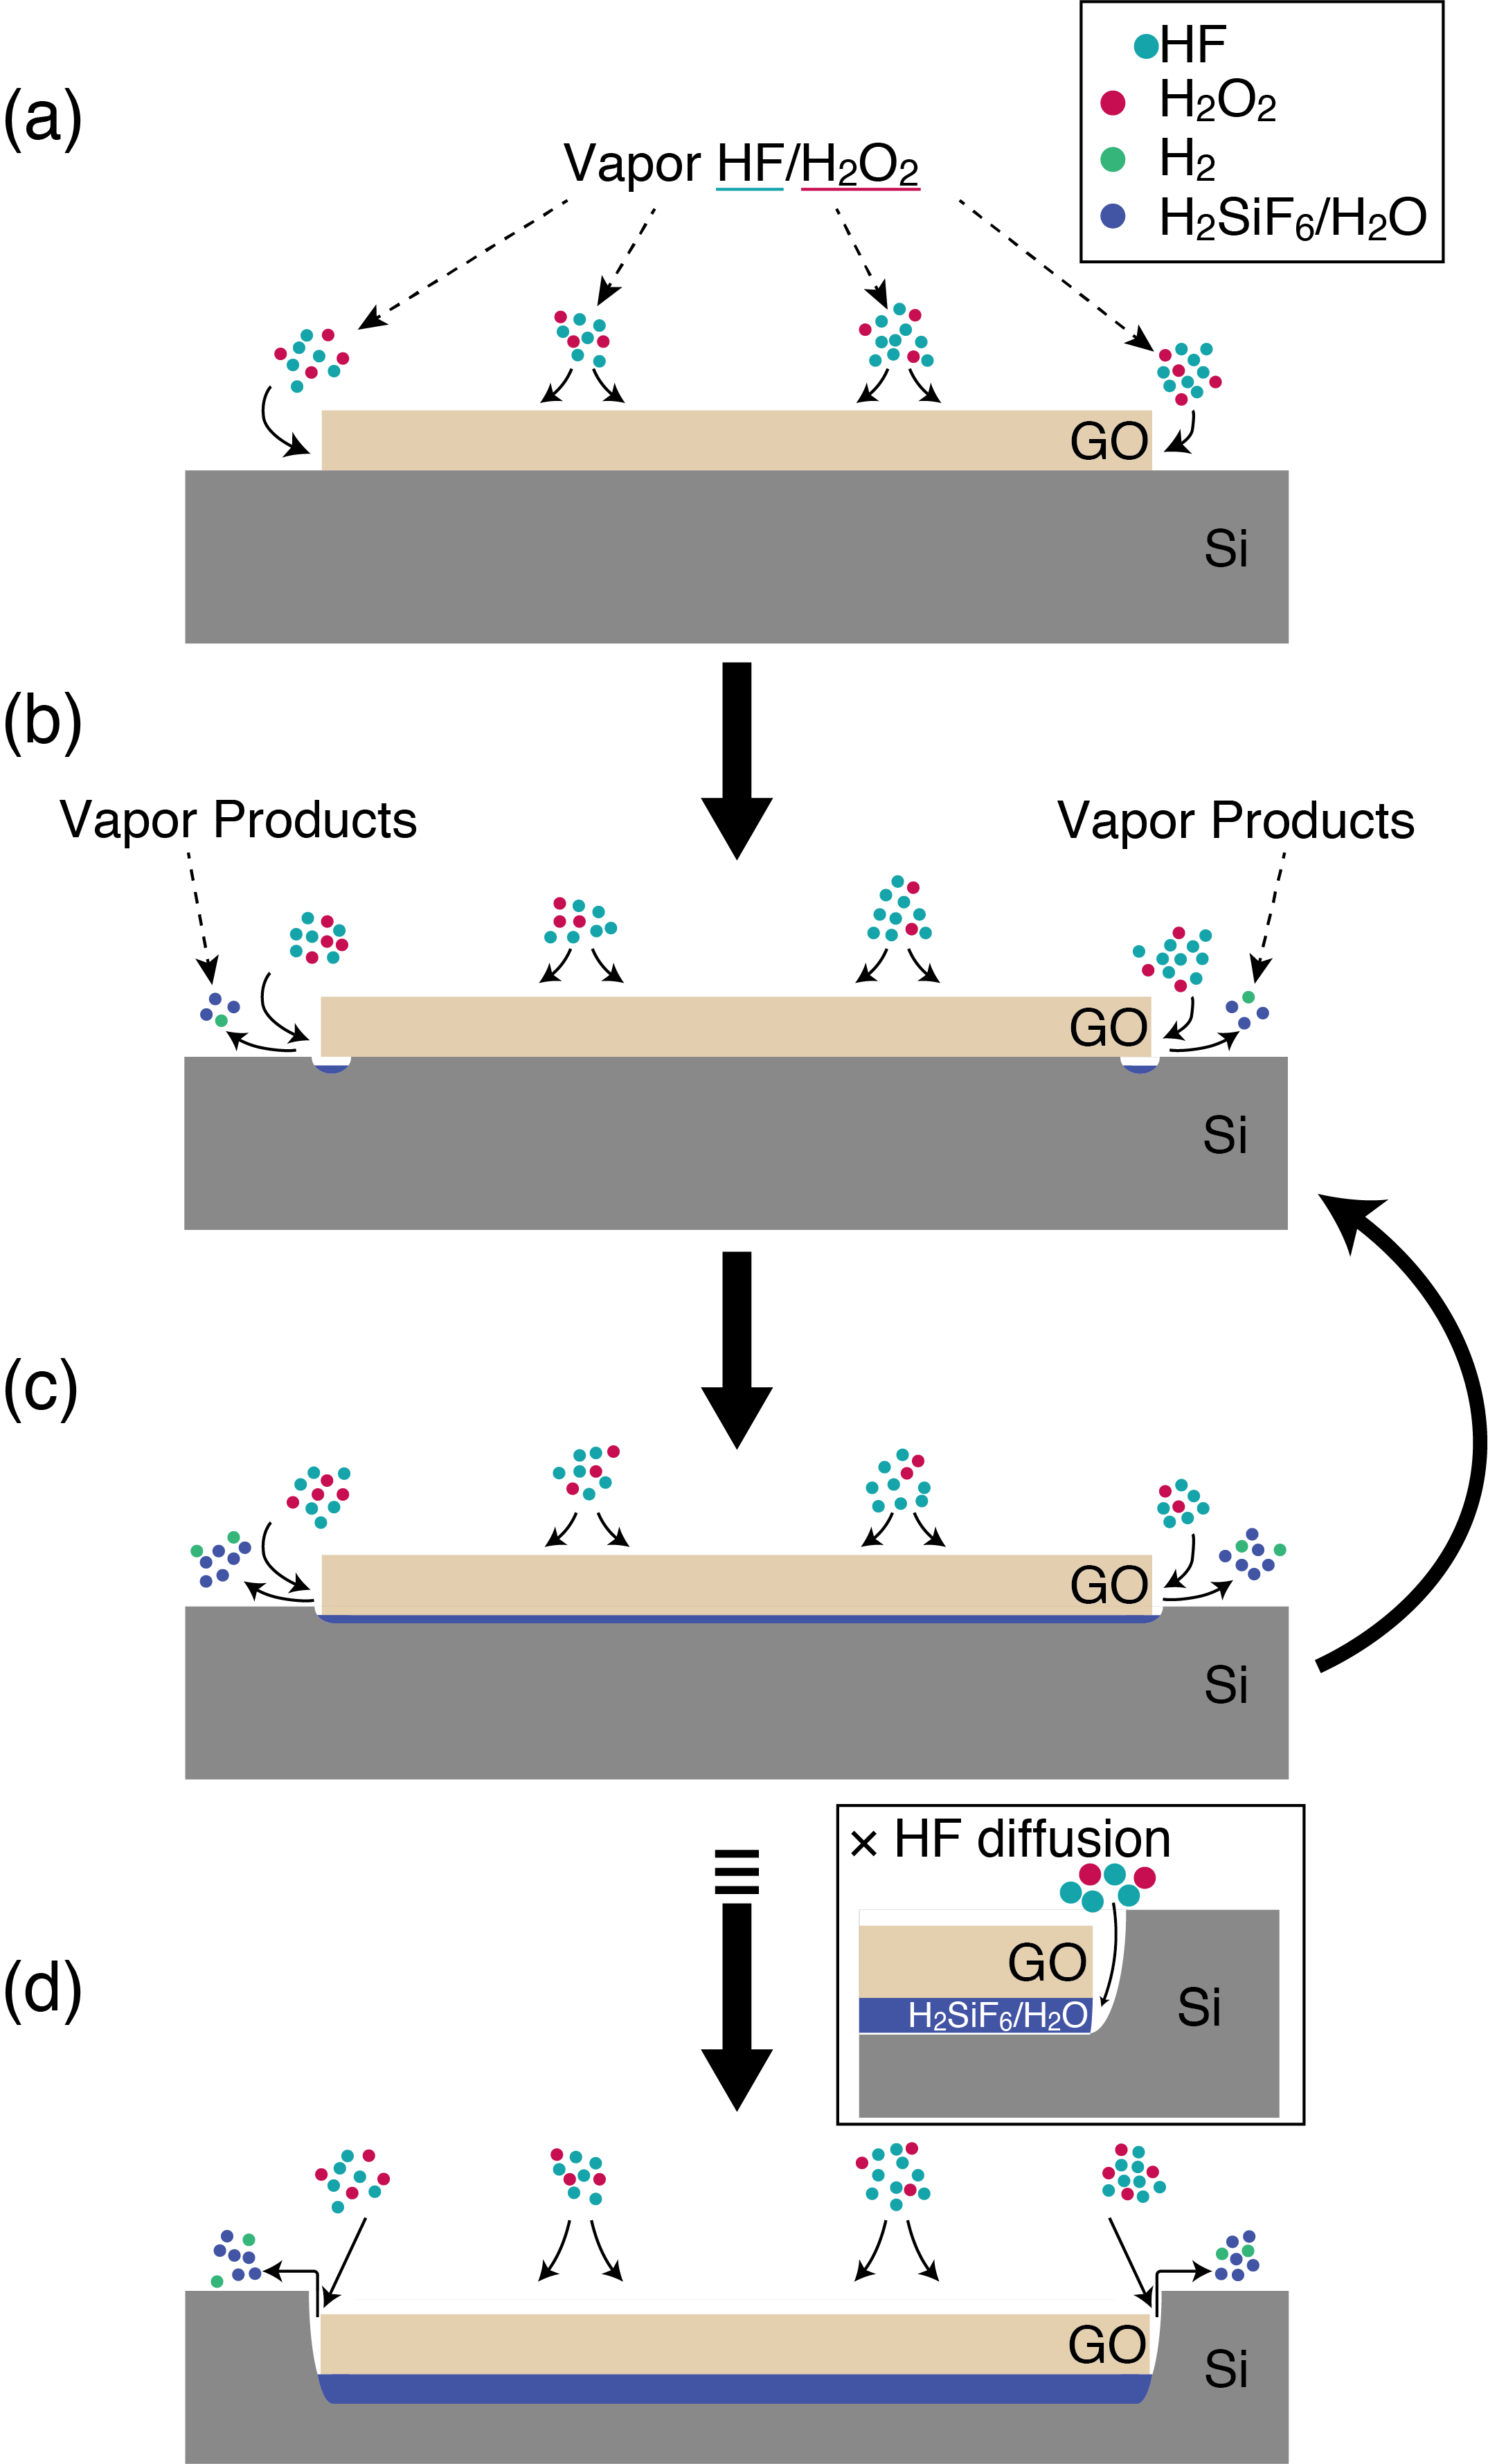
\includegraphics[width=100mm]{figures/figure9.png}
%     \caption{Schematic illustrations of the mechanism of the vapor-etching with GO.}
%     \label{fig:Schematic_mechanism}
% \end{figure}

Fig.\ref{fig:SEM}は50 ${}^\circ$Cで16時間エッチングを行った後のGOが担持されたシリコン基板のSEM像である.
Fig.\ref{fig:SEM}(a-1),(a-2)からわかるようにGOが担持されていないベアシリコン部が"島"として存在していることが改めてわかった.
Fig.\ref{fig:SEM}(b-1),(b-2),(b-3)はそれぞれGO,rGO,rGO\_140を用いてエッチングを行った後の断面SEM像である.
どの試料においても,GO直下のシリコンが優先的に溶解しているだけでなく,ベアシリコン部において,ナノ・メソスケールのポーラス構造の形成が観察されなかった.



\begin{figure}[H]
    \centering
    \includegraphics[width=175mm]{figures/figure10.png}
    \caption{(a-1) A SEM image of the silicon substrate loaded with rGO\_140 after vapor-phase etching at 50 ${}^\circ$C for 16 h. (a-2) shows the higher magnification SEM image. Cross-sectional SEM images of the etched silicon loaded with (b-1) GO, (b-2) rGO, and (b-3) rGO\_140 at 50 ${}^\circ$C for 16 h.}
    \label{fig:SEM}
\end{figure}

\section*{\ul{Conclusion}}
本実験から,GOを用いた気相シリコンエッチングでは酸化剤還元反応が律速過程である可能性が高いことがわかった.
また,酸化剤還元を大きく促進するのは,GOシート面内のエッジや空孔といったVUV光還元によって修復されない欠陥であることが示唆された.
さらに液相と気相で,GOがエッチングを促進するメカニズムが異なることも明らかとなった.

\section*{\ul{Future plan}}
\begin{enumerate}
    \item 酸化剤濃度のエッチング挙動への影響をより詳しく明らかにする.
    \item GOの層数がエッチング挙動に与える影響について明らかにする.
    \item 赤外ランプ加熱を用いて,高温(\~ 800 ${}^\circ$C)下で加熱する処理をVUV光照射と組み合わせて,より構造欠陥の少ないrGOの作製を目指す.
    \item n型シリコン基板でのエッチング挙動について,p型シリコンの場合と差異があるのか明らかにする.
    \item Mott-Schottky プロットを取ることで,実際のエッチャントの仕事関数を求める?.
    \item 欠陥の中でも,どの欠陥が酸化剤還元反応を促進しているのか理論計算を行う?
\end{enumerate}

\section*{\ul{Appendix}}
Fig.\ref{fig:appendix1}はGOを用いたシリコンアシストエッチングのメカニズムを説明する模式的なバンド図である.
Fig.\ref{fig:appendix1}(a)はフッ酸とp型シリコンの接触前のバンド図であり,$E_{Fm}$はフッ酸のフェルミ準位,$E_{C}$,$E_{V}$,$E_{Fs}$はそれぞれp型シリコンの伝導帯,価電子帯,フェルミ準位である.
まずGOがシリコン基板に担持されていない場合での接触を考える(Fig.\ref{fig:appendix1}(b)).
Macetchにおいて,触媒金属とフッ酸溶液(もしくはフッ酸・過酸化水素混合溶液)を電極とみなし,Poissonおよび drift-diffusion方程式をself-consistentに解き,バンドオフセットを求めたシミュレーションは既に何件か報告されている\supercite{torralba_tunable_2016, pinna_mesopore_2020, matsumoto_composite_2022}.
これまでの報告では,フッ酸とp型シリコン界面では欠乏層が形成されており(Fig.\ref{fig:appendix1}(b) left),過酸化水素や硝酸といった酸化剤の添加がp型シリコンの陽極酸化の役割(バイアス:$\Psi$)を果たす(Fig.\ref{fig:appendix1}(b) right),つまり蓄積層を形成するとされてきた\supercite{torralba_tunable_2016, pinna_mesopore_2020, matsumoto_composite_2022}.
\indent
GOがシリコンに担持された場合も,同様に考えることができると推測される.
GOはその厚さ($\delta$)が1 nmほどであるため,フッ酸溶液とp型シリコン間をキャリアはトンネル効果によって移動することができ,両者のフェルミ準位は一致すると推測される(Fig.\ref{fig:appendix1}(c) left).
ここで酸化剤を添加するとFig.\ref{fig:appendix1}(b) rightと同様に陽極酸化が起こる.
GOは酸化剤還元を促進するため\supercite{kubota_chemical_2019, kubota_chemical_2021},その分に相当する電圧($V$)がさらにp型シリコンに印加されると予測される(Fig.\ref{fig:appendix1}(c) right),すなわち$\Psi + V$ (V > 0).
ベアシリコンと比較して,GO担持シリコンではその正孔濃度が大きいため(正孔濃度は$E_F - E_V$ に指数関数的に比例する)ため,GO直下のシリコンが優先的に溶解する現象が観察されると推測される.

\begin{figure}[H]
    \centering
    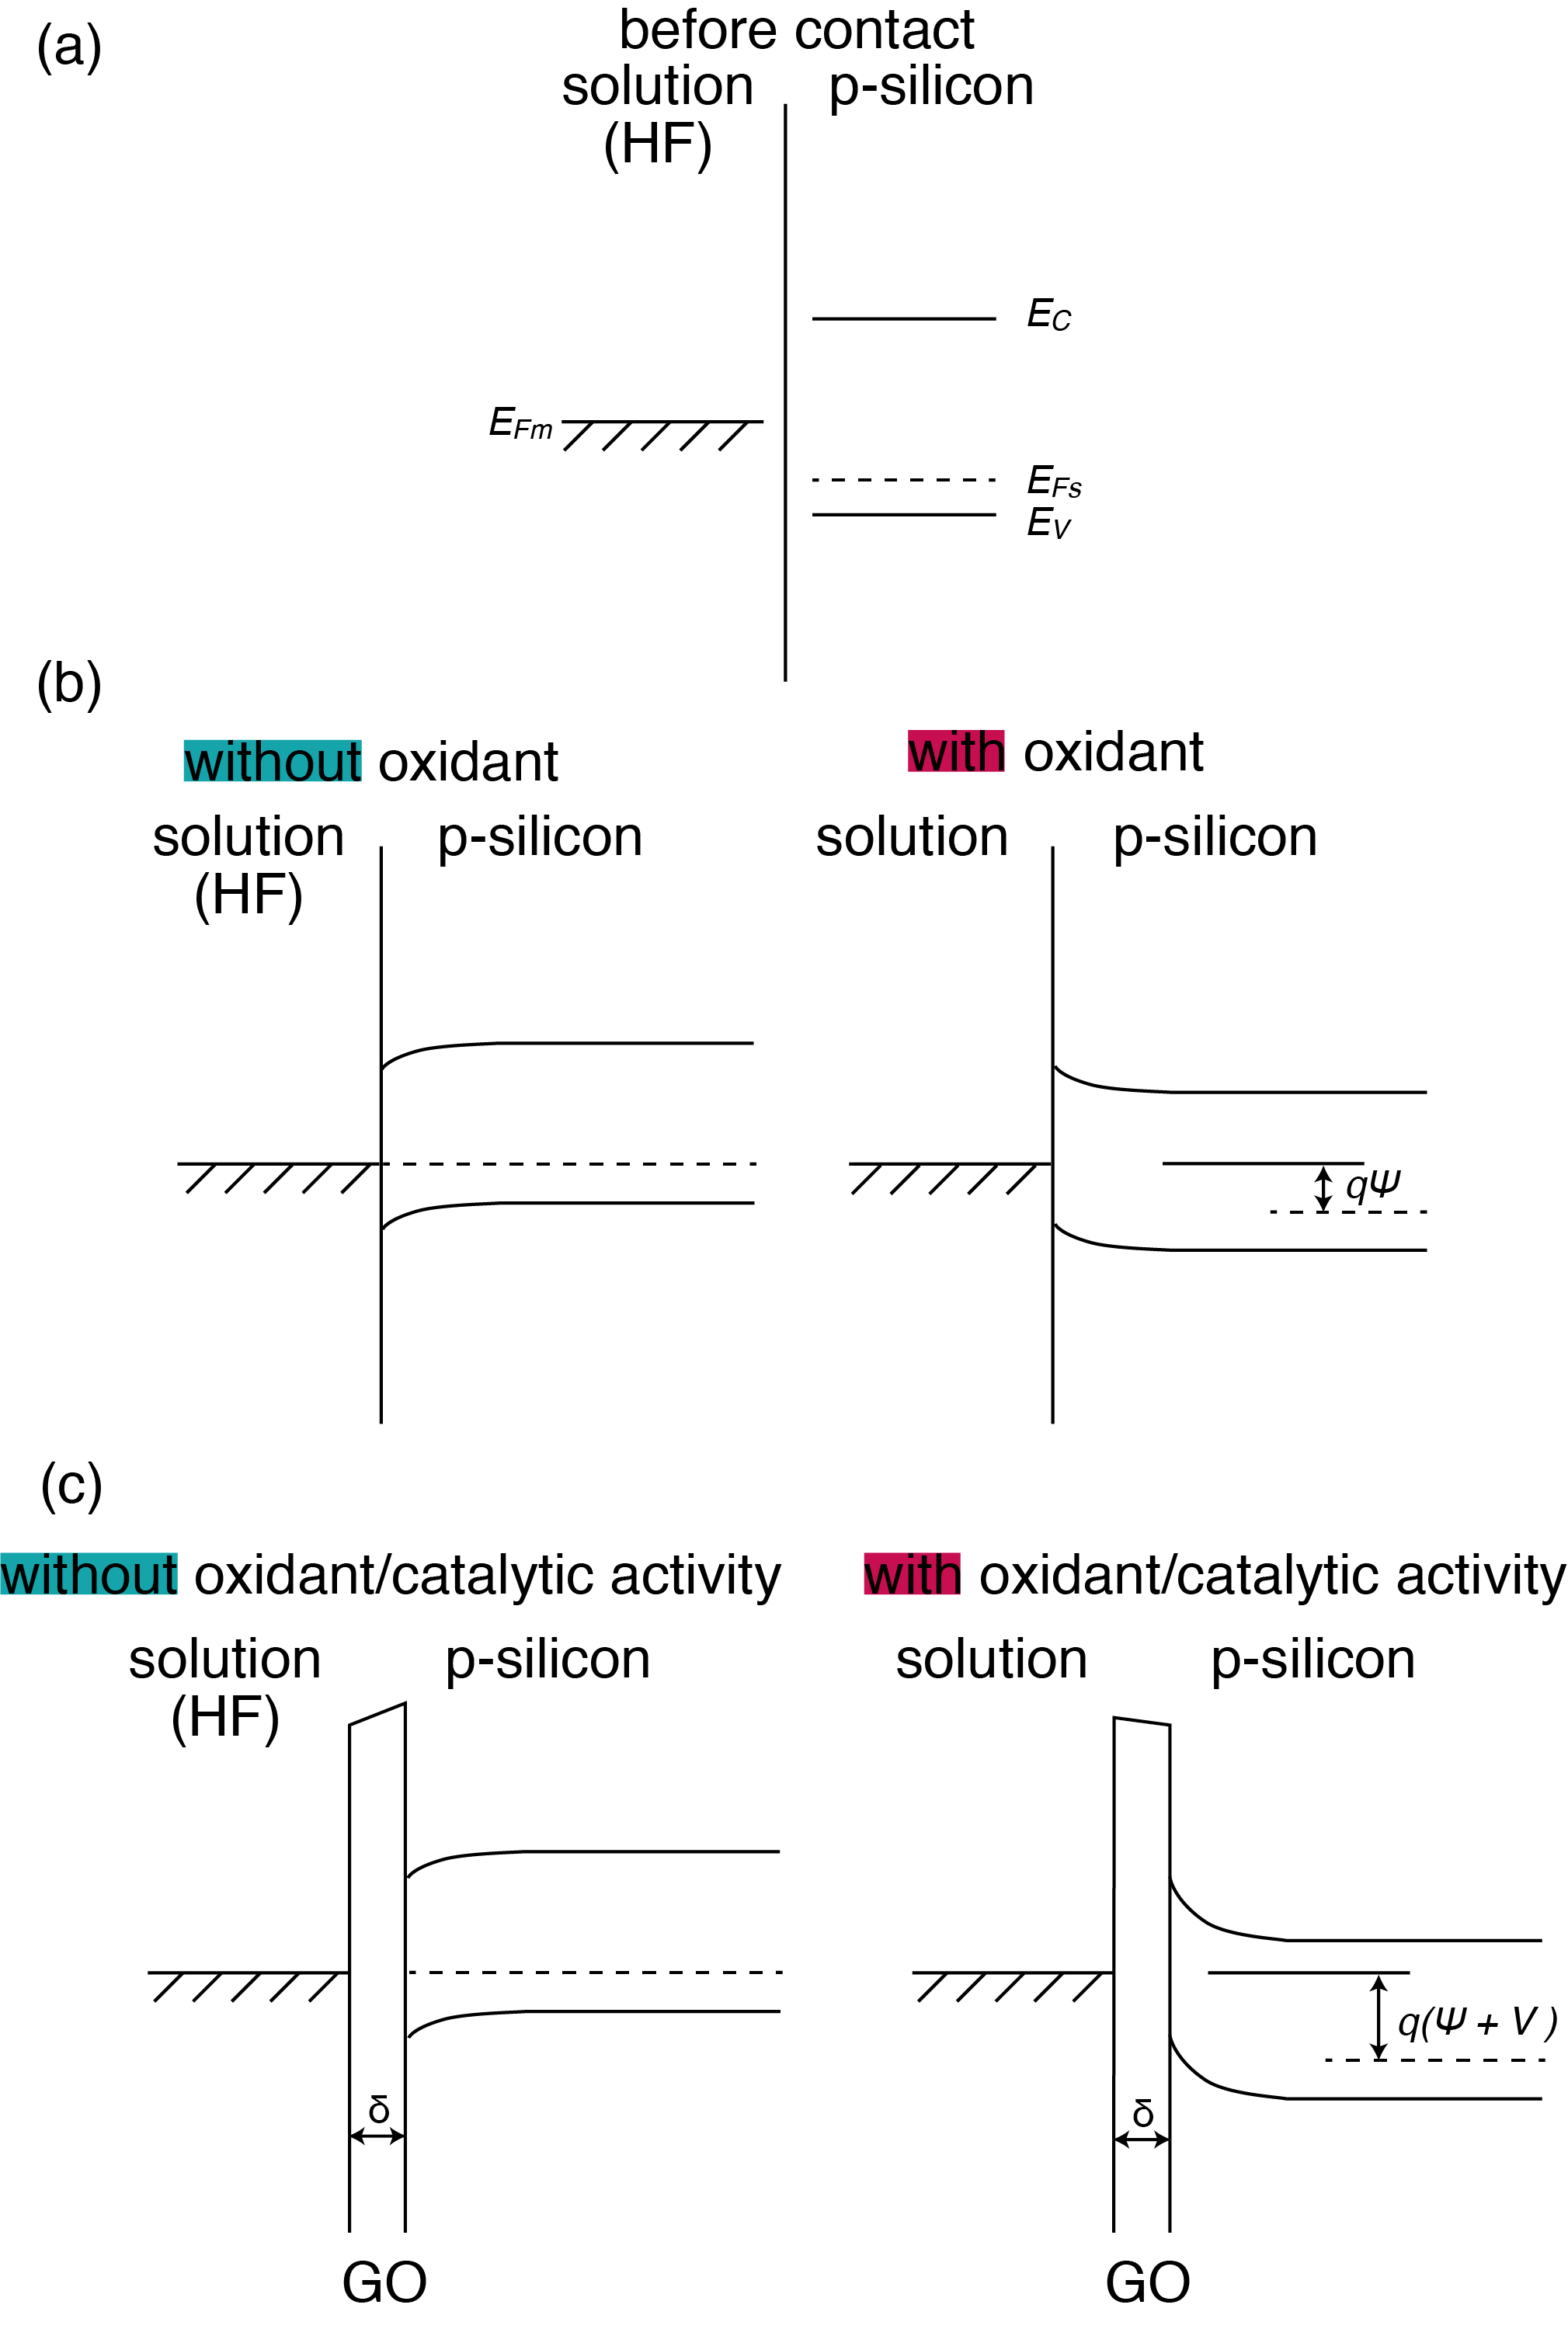
\includegraphics[width=100mm]{figures/appendix1.png}
    \caption{Schematic band diagrams of solution (HF) and p-doped silicon. Their respective band diagram before the contact is shown in (a). The band alignment of HF/p-doped silicon without or with GO is shown in (b) or (c), respectively.}
    \label{fig:appendix1}
\end{figure}

\newpage
\printbibliography

\end{document}